\newpage

\section{SSA-Style optimizations}

\subsection{Constant Propagation}
\begin{note}{notes}
	\begin{itemize}
		\item If  v $\gets$ c , replace all uses of v with c
		\item If  v $\gets$  $\Phi$ (c,c,c)  (each input is the same constant), replace all uses of v with c
	\end{itemize}
\end{note}


\begin{algorithm}
	\caption{SSA-CP}\label{alg:SSA-CP}
	\begin{algorithmic}
		\State{W $\gets$ list of all defs}
		\While{!W.isEmpty()}

		\State{Stmt S $\gets$ W.removeOne()}
		\If{(S has form v $\gets$ c) or
			(S has form v $\gets$ $\Phi$(c,...,c))}
		\State delete S
		\For{each stmt U that uses v}
		\State {replace v with c in U}
		\State {W.add(U)}
		\EndFor
		\EndIf
		\EndWhile

	\end{algorithmic}
\end{algorithm}

\subsection{Conditional Constant Propagation }

In this section, we want to talk something about Conditional Constant Propagation. 
Before we talk about it, we need to know something about the history of Constant Propagation.
There are four algorithms for determining constants.
 They are described in order of increasing power; each algorithm finds at least the
constants found by the previous algorithm. These algorithms are among the
simplest, fastest, and most powerful global constant propagation algorithms
known. The first three algorithms are reformulations of the work of others;
the fourth is new and contains the best features of each of the previous three.
Figure \ref{fig:p223} shows the relationship among the four algorithms.


\begin{figure}[H]
	\centering
	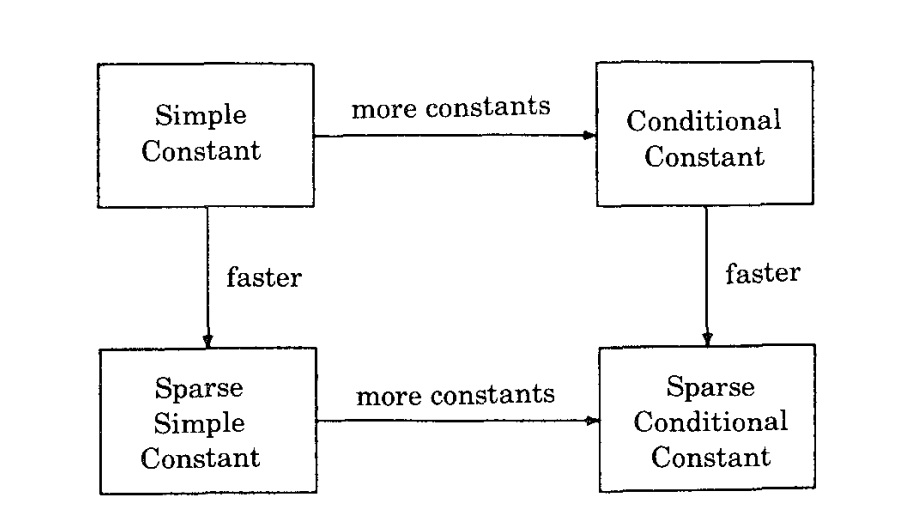
\includegraphics[width=0.5\textwidth]{p223.png}
	\caption{Relationship among the four constant propagation algorithms}
	\label{fig:p223}

\end{figure}


The first algorithm, Simple Constant (SC), was developed by Kildall\cite{kildall1973unified}. 
Kildall was among the first to describe the
constant propagation problem and to give an algorithmic solution.



The second algorithm, Sparse Simple Constant (SSC), is an easily understood reformulation of an algorithm developed by Reif and Lewis\cite{reif1977symbolic}. 
This algorithm uses a data
structure called the static single assignment graph (SSA graph). The SSA
graph is a variant of the global value graph of Reif and Lewis, which in
turn is based on the p-graph of Shapiro and Saint. The SSA graph allows
this algorithm to find a class of constants equivalent to those of SC, yet the
algorithm is faster than SC by a factor proportional to the number of
variables in the program. Indeed, the speedup can be proportional to the
product of the number of variables in the program and the number of edges
in the program flow graph. It is unfortunate that this algorithm was not
recognized for many years, since it works in time linear in the size of the SSA
graph.


The third algorithm, Conditional Constant (CC), is a variant of Wegbreit’s
Algorithm\cite{wegbreit1975property}. CC discovers all constants
that can be found by evaluating all conditional branches with all constant
operands, but it uses the same input data structures and is asymptotically as
slow as SC. The attraction of CC is that it propagates the values in such a
way that when conditional branches are found to have a constant conditional
expression, the search for constants can ignore parts of the program that are
never executed. The algorithm does unreachable code elimination in combination with constant propagation. 
The first benefit of this approach is that
the algorithm may run faster than SC, since it need not evaluate the sections
of the program that are never executed. A second benefit is that values
created in the unreachable areas cannot possibly kill potential constants, and
thus CC can find more constants than can SC.

The fourth algorithm, Sparse Conditional Constant (SCC) finds the same class of constants as CC, yet has
the same speedup over CC as SSC has over SC.


Wegman and Zadeck's Sparse Conditional Constant (SCC) algorithm was used to find constant expressions, 
constant conditions, and unreachable code \cite{wegman1991constant}. The output of the SCC algorithm is 
an association of variables to one of $\lbrace \bot, c, \top \rbrace$, where $\bot$ marks a variable that
 can hold different values at different times, and $\top$ means the variable is not executed. In addition, 
 every flow-graph node (corresponding to a quadruple) is marked as executable or non-executable. 
 We then walk the flow-graph, eliminating dead-code (quadruples marked non-executable), replacing 
 constant variables with their values, and changing constant conditional branches to goto statements.

\begin{note}{notes}
	\begin{itemize}
		\item Assume all blocks unexecuted until proven otherwise
		\item Assume all variables are not executed (only with proof of assignment of a non-constant value do we assume not constant)
	\end{itemize}
\end{note}

\subsubsection{Example}

\begin{figure}[H]
	\centering
	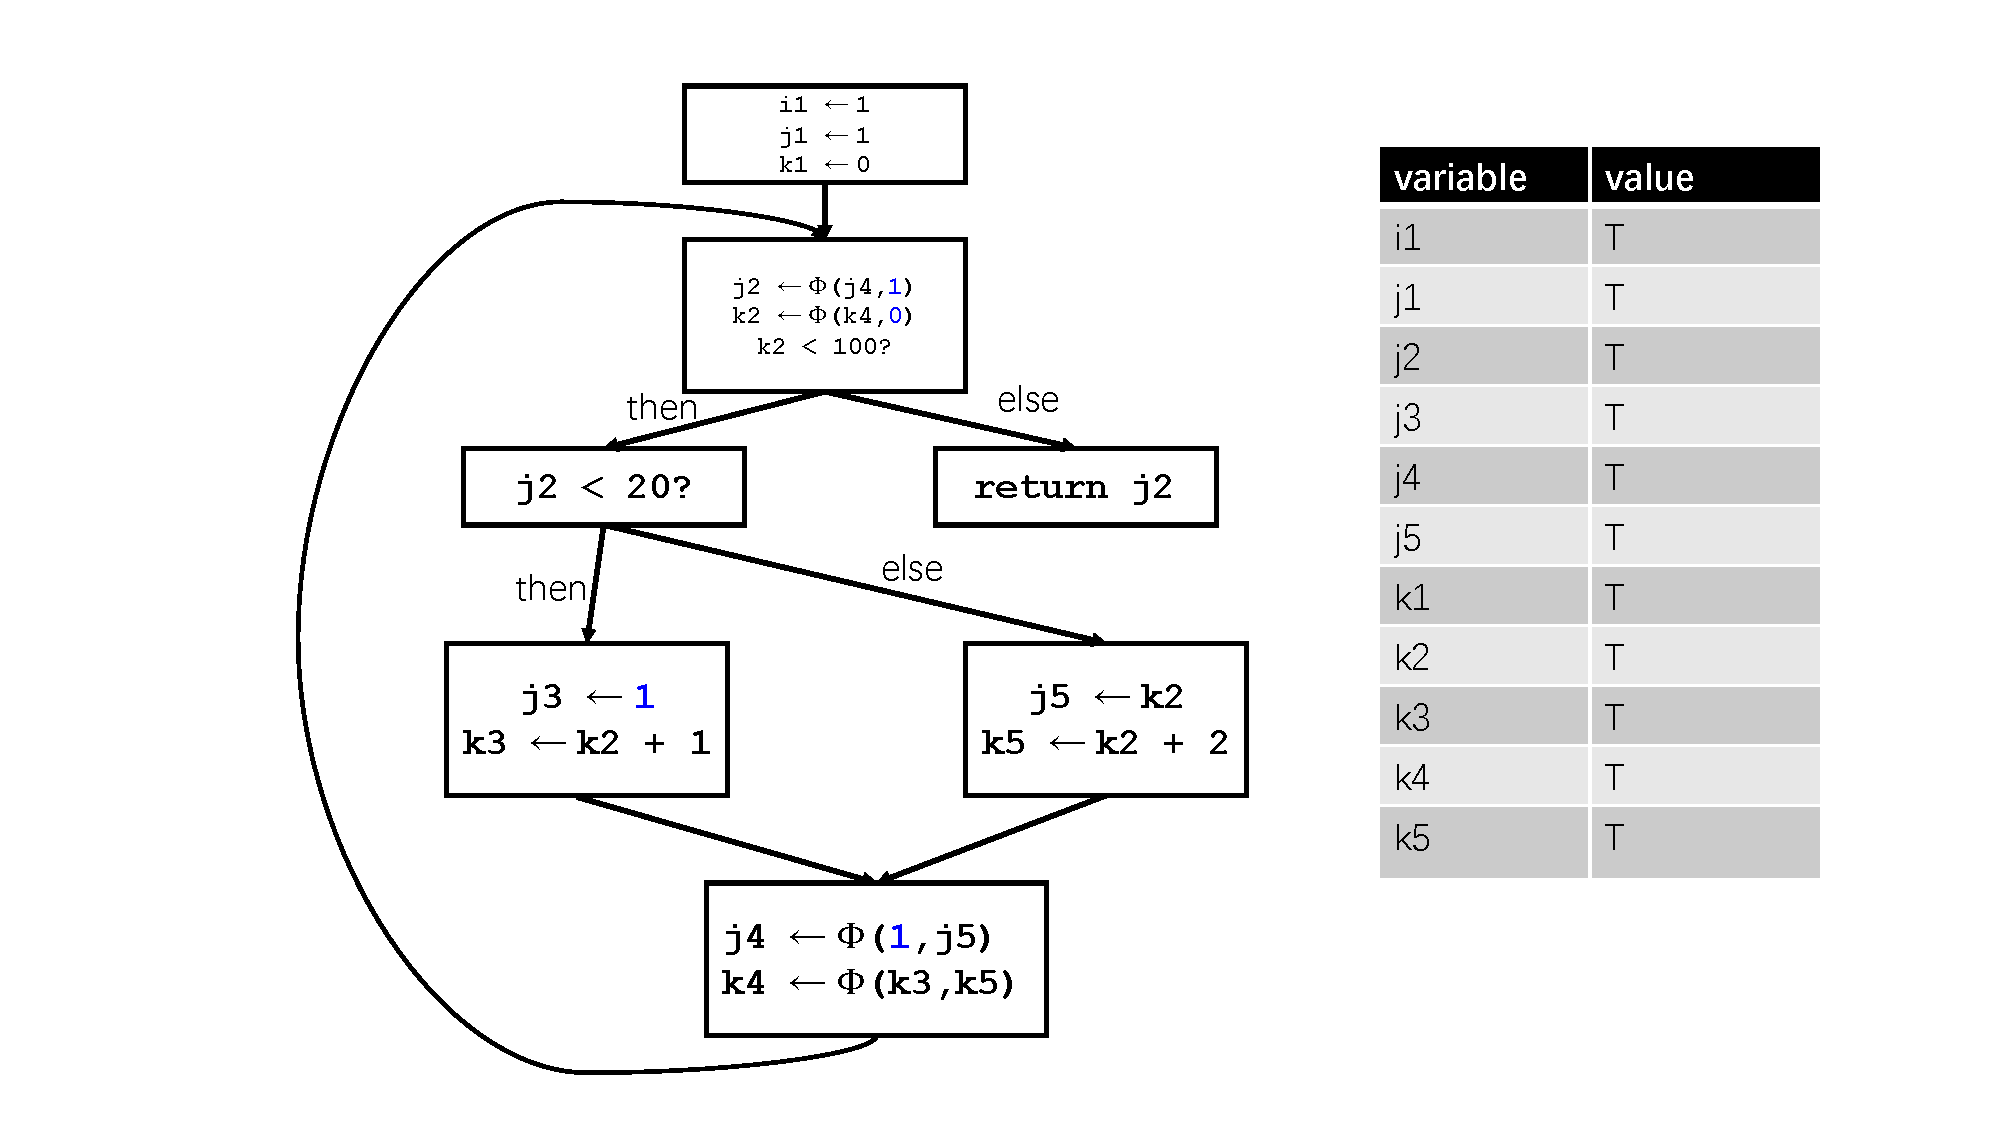
\includegraphics[width=\textwidth]{p47.pdf}
	\caption{Original code. The black block is marked as unexecuted}
	\label{fig:p47}

\end{figure}




\begin{figure}[H]
	\centering
	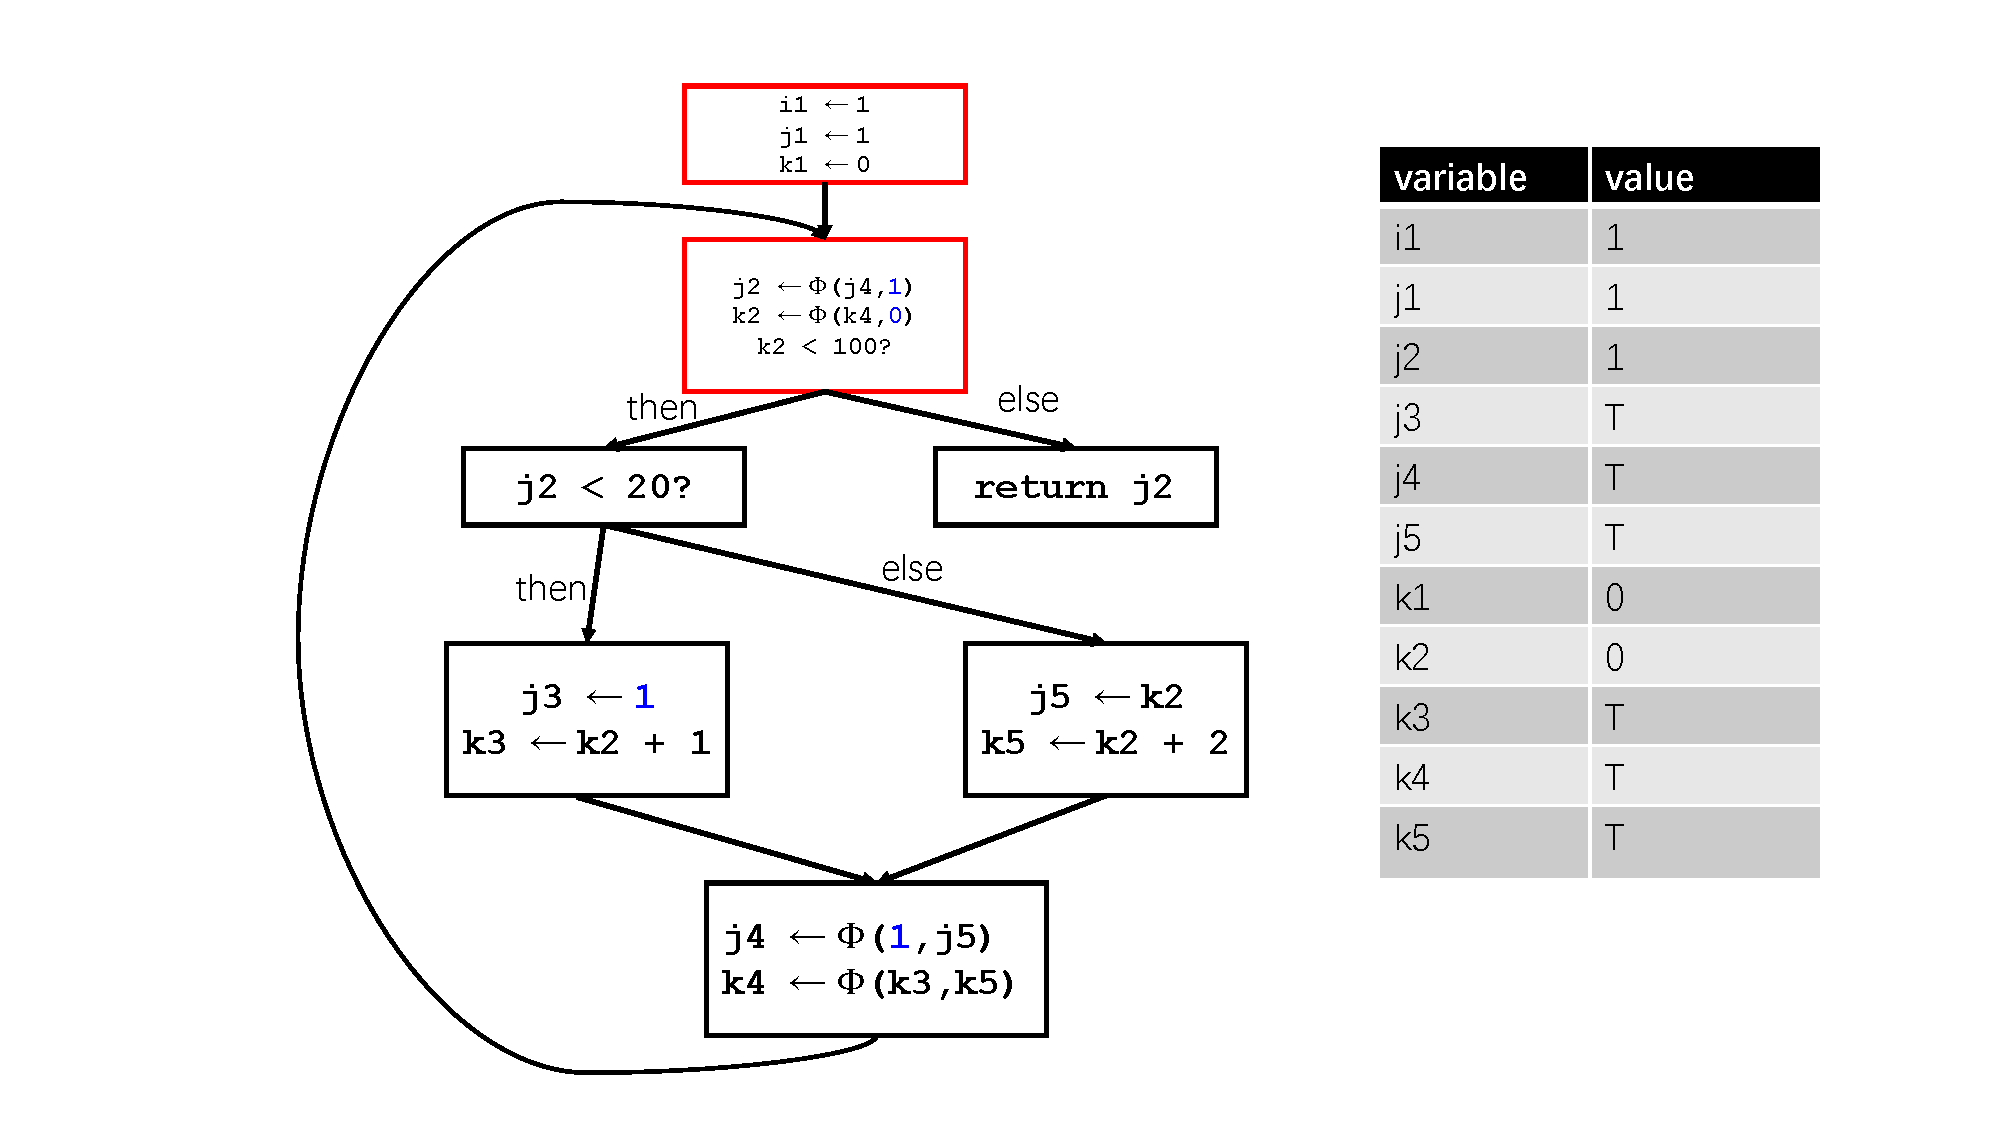
\includegraphics[width=0.8\textwidth]{p48.pdf}
	\caption{The read block is marked as executed. After walking the first two blocks, the value is shown above.}
	\label{fig:p48}

\end{figure}



\begin{figure}[H]
	\centering
	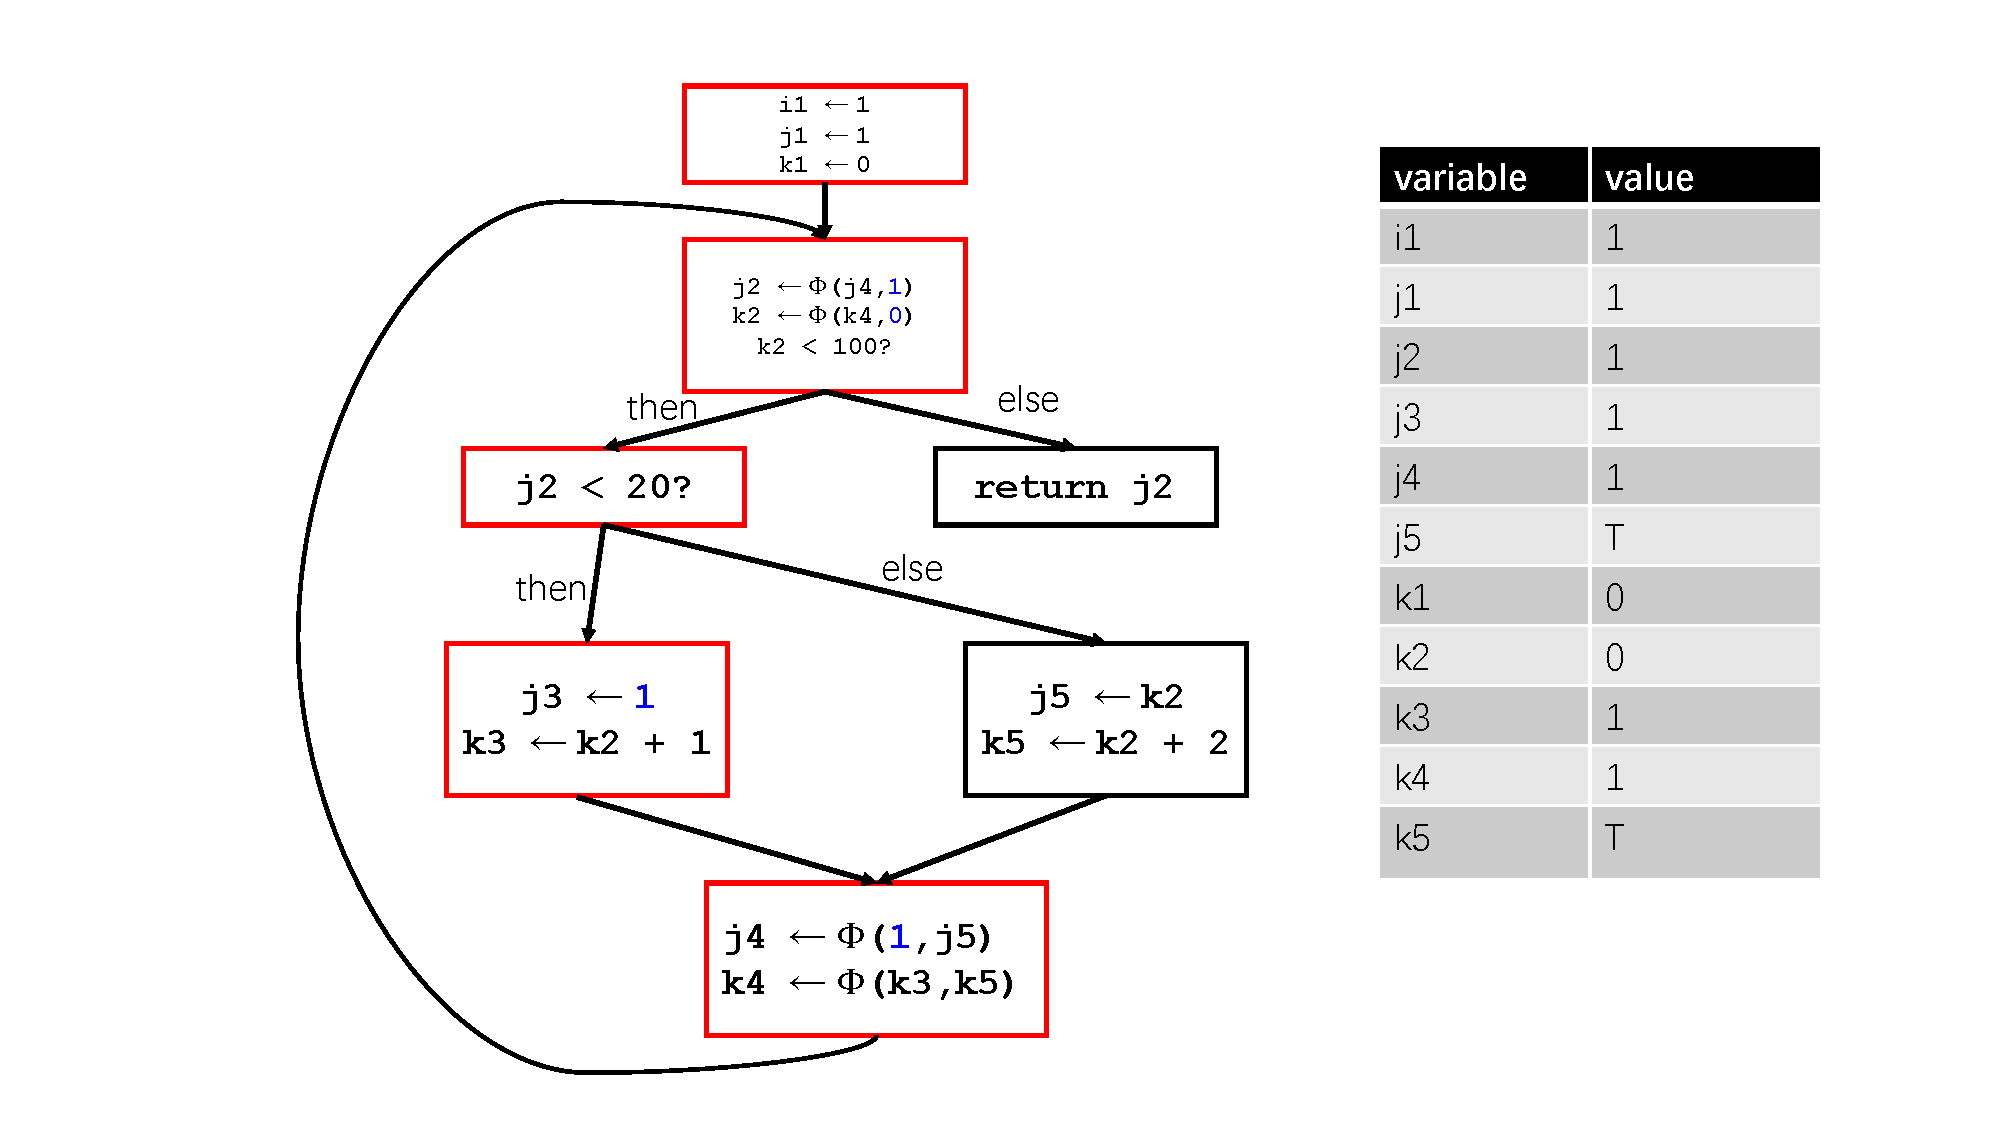
\includegraphics[width=0.8\textwidth]{p49.pdf}
	\caption{After walking 5 blocks.}
	\label{fig:p49}

\end{figure}



\begin{figure}[H]
	\centering
	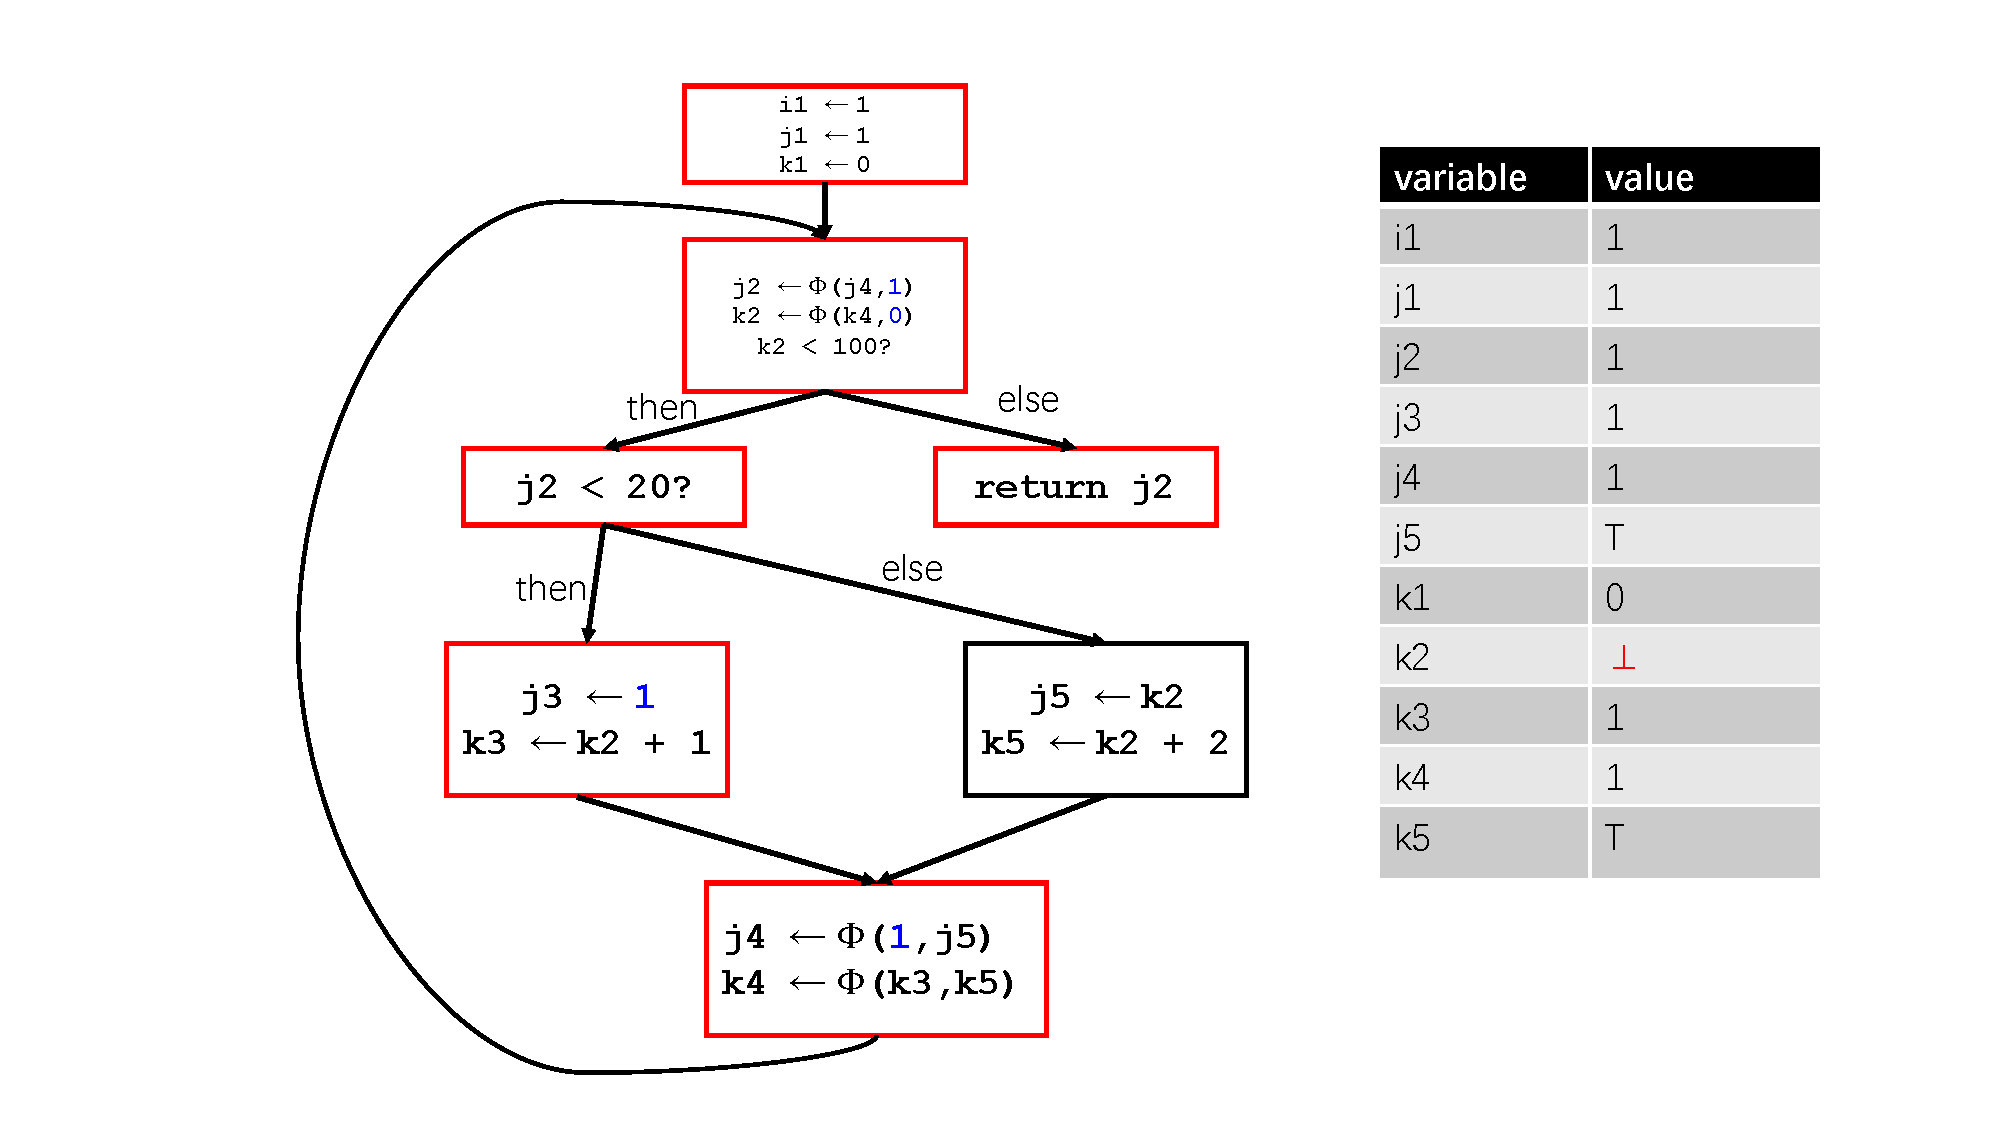
\includegraphics[width=0.8\textwidth]{p50.pdf}
	\caption{Now k2 is $\bot$, so the \texttt{return j2} is reachable.}
	\label{fig:p50}

\end{figure}



\begin{figure}[H]
	\centering
	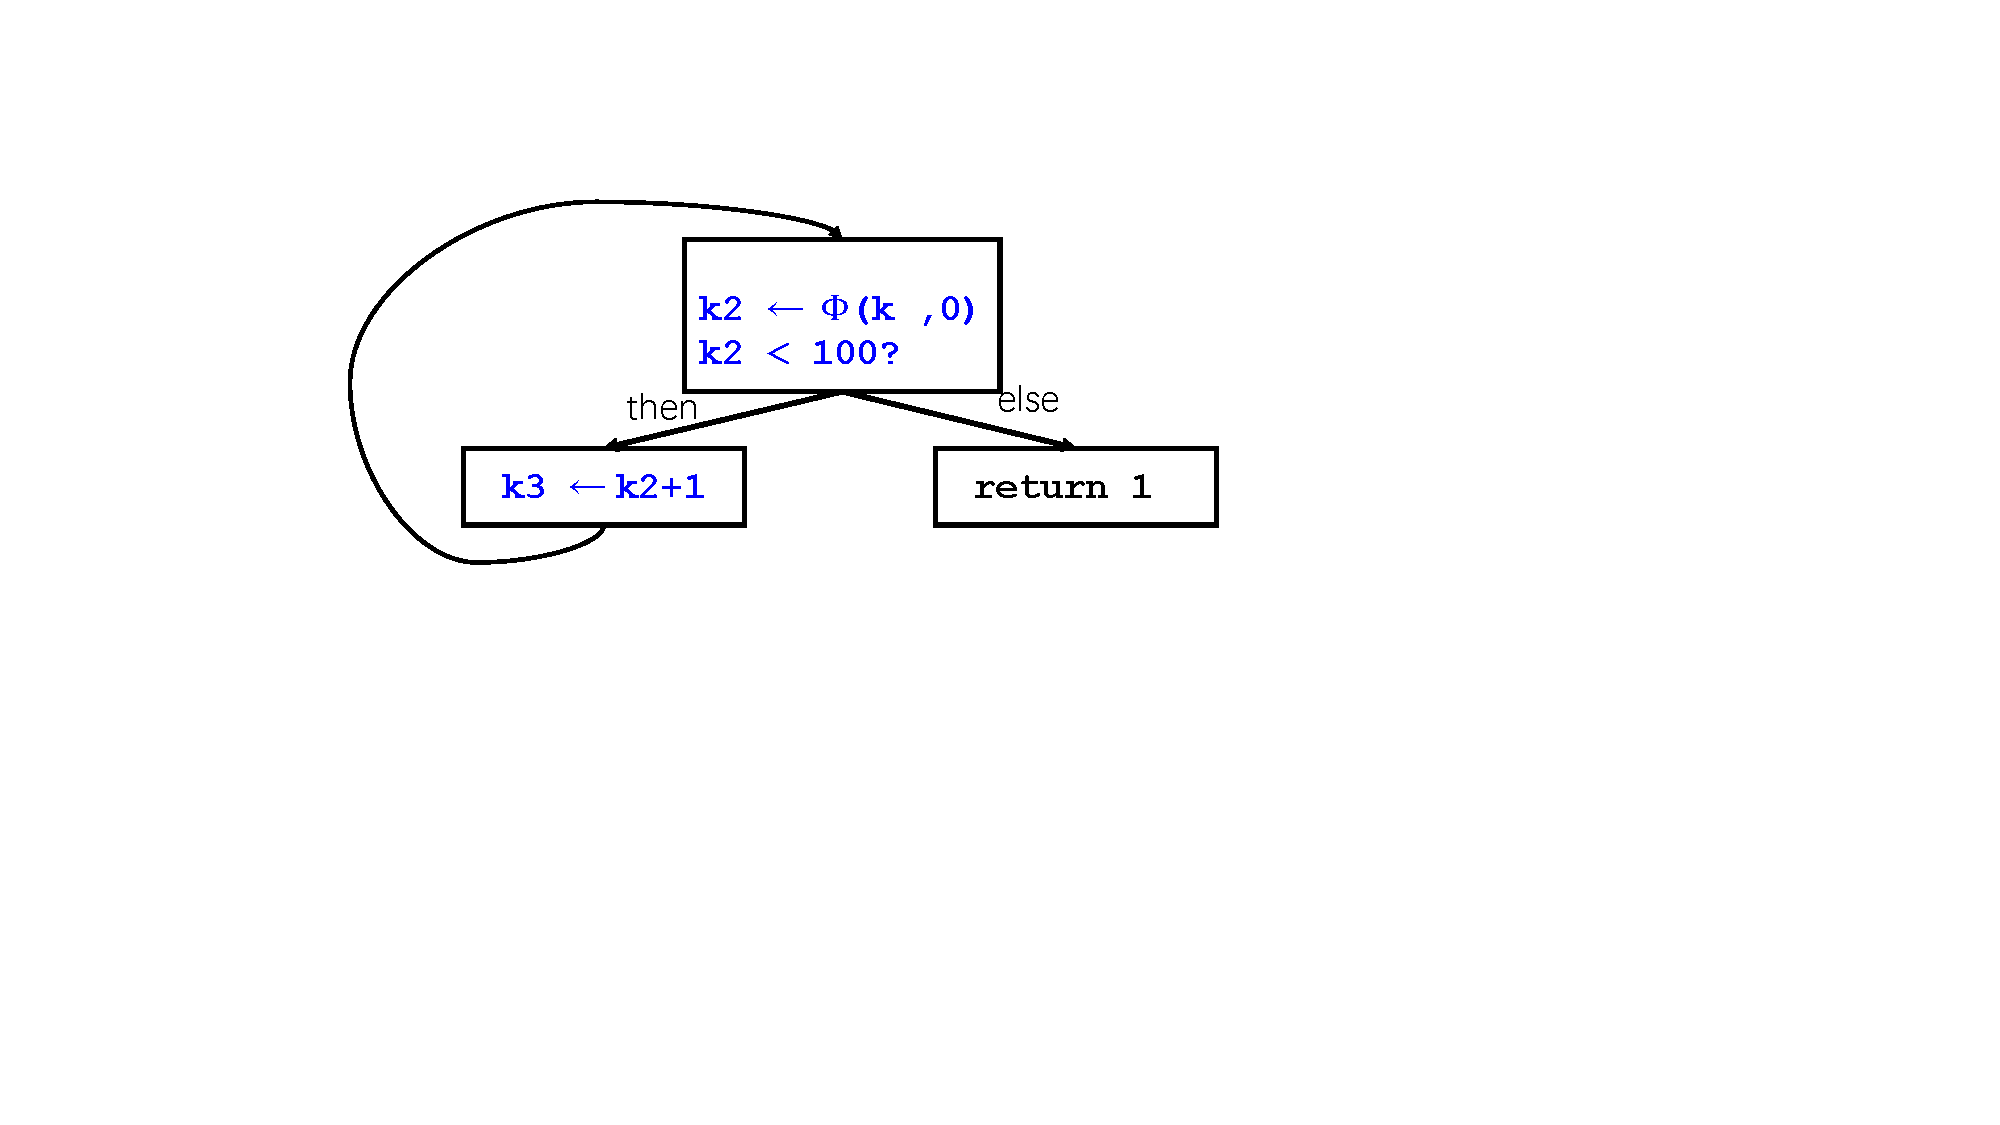
\includegraphics[width=0.5\textwidth]{p51.pdf}
	\caption{Code after applied SCC.}
	\label{fig:p51}

\end{figure}


% \begin{figure}[!b]
%      \centering
%      \begin{subfigure}{0.45\textwidth}
%      \centering
%          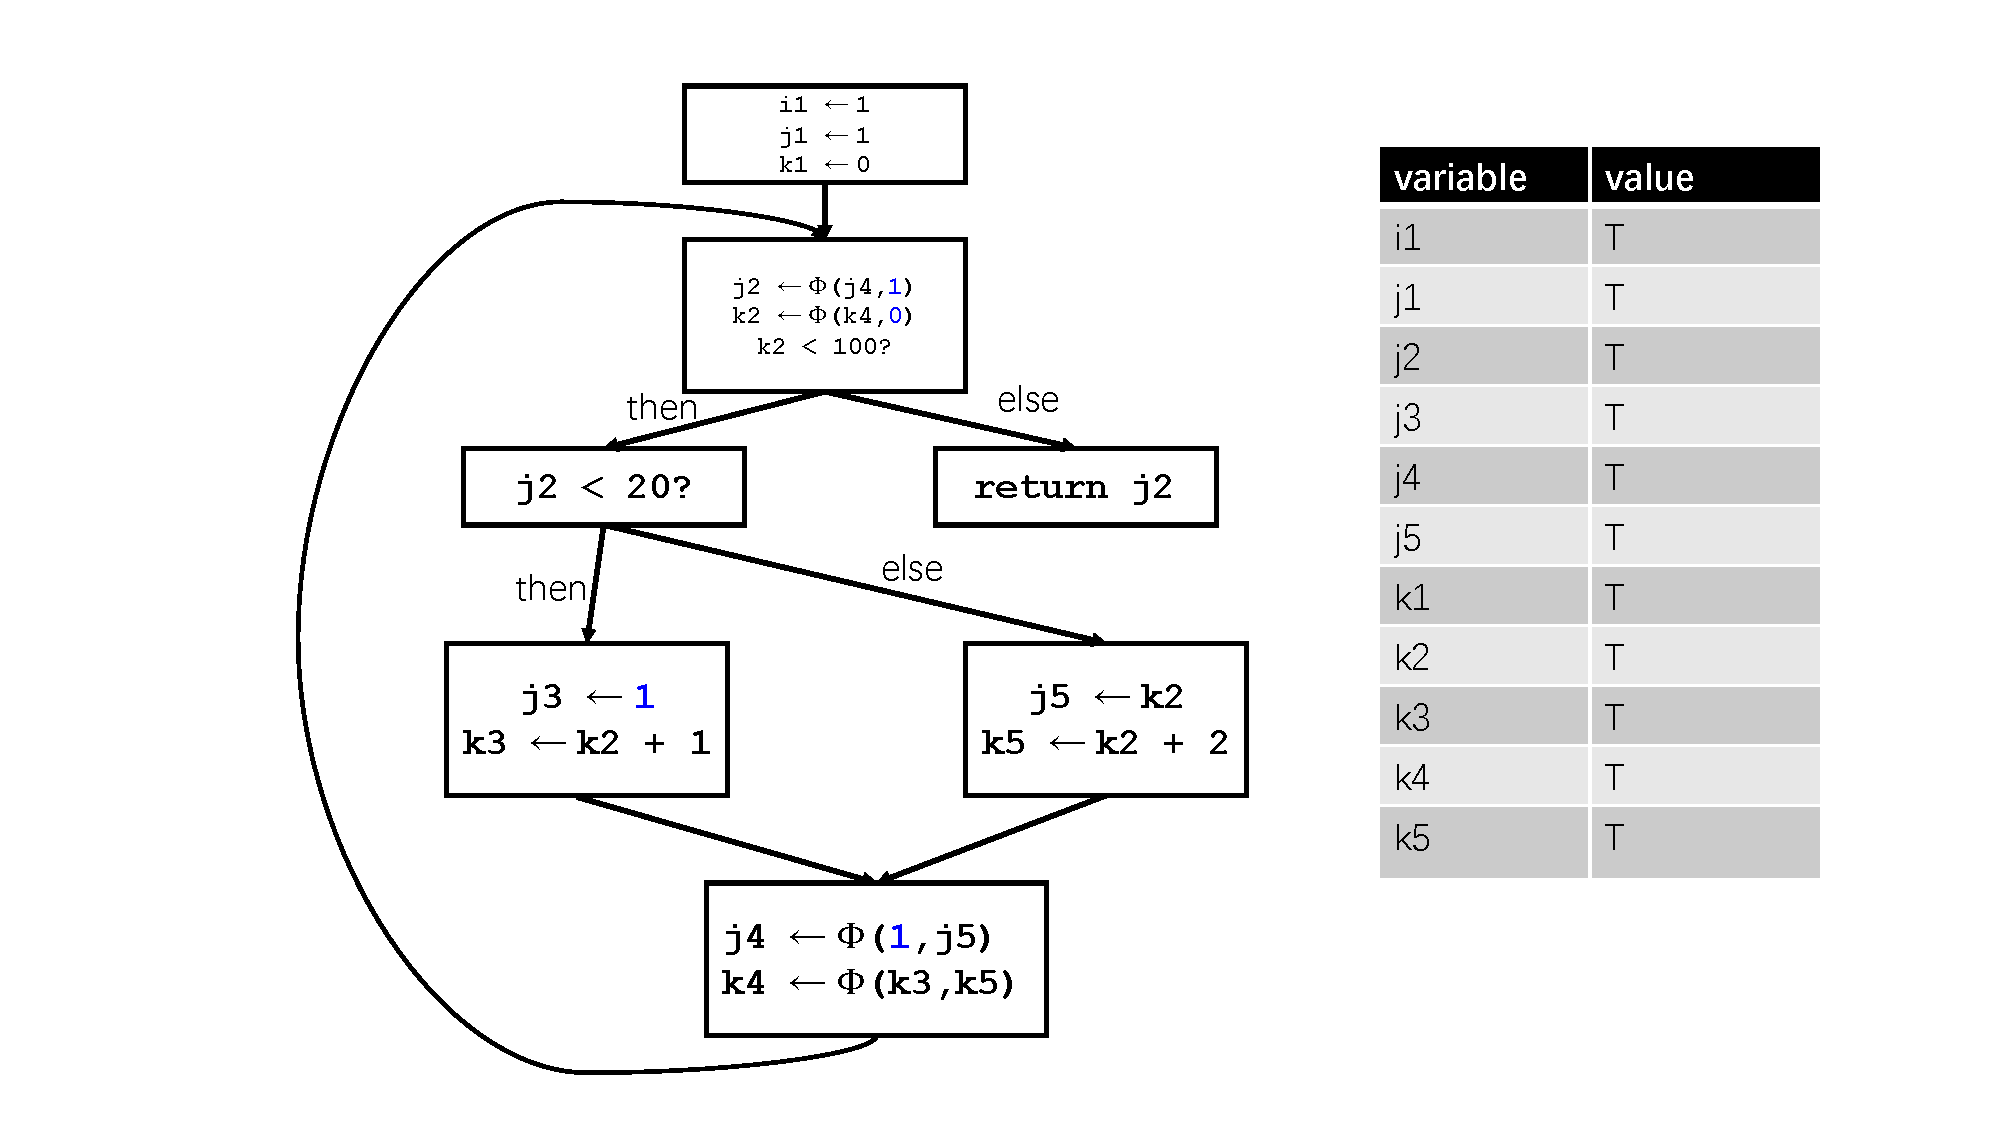
\includegraphics[width=\textwidth]{p47.pdf}
%          \caption{Original code}
%          \label{fig:p47}
%      \end{subfigure}
%      \begin{subfigure}{0.6\textwidth}
%      \centering
%          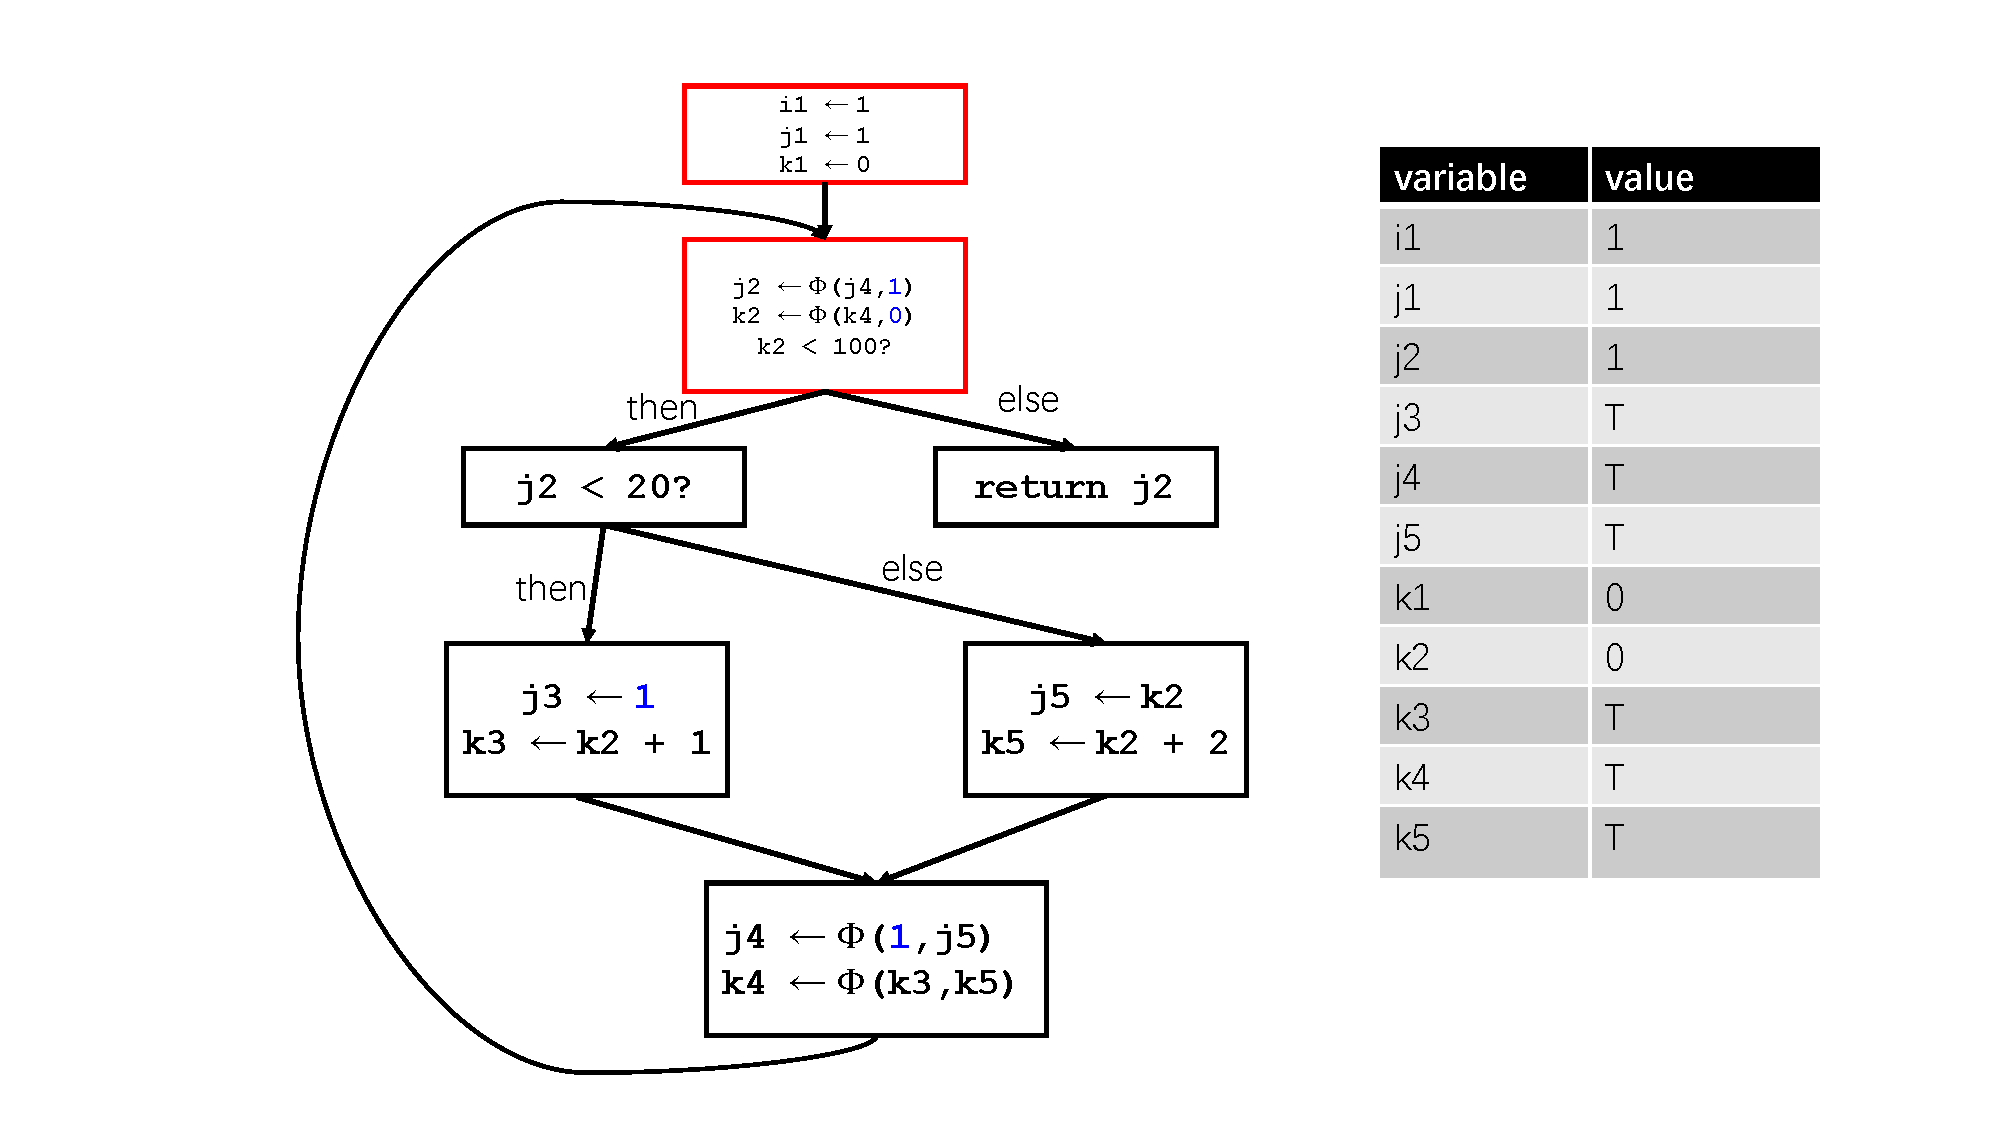
\includegraphics[width=\textwidth]{p48.pdf}
%          \caption{Code after moving instruction.}
%          \label{fig:p48}
%      \end{subfigure}
%           \begin{subfigure}{0.6\textwidth}
%      \centering
%          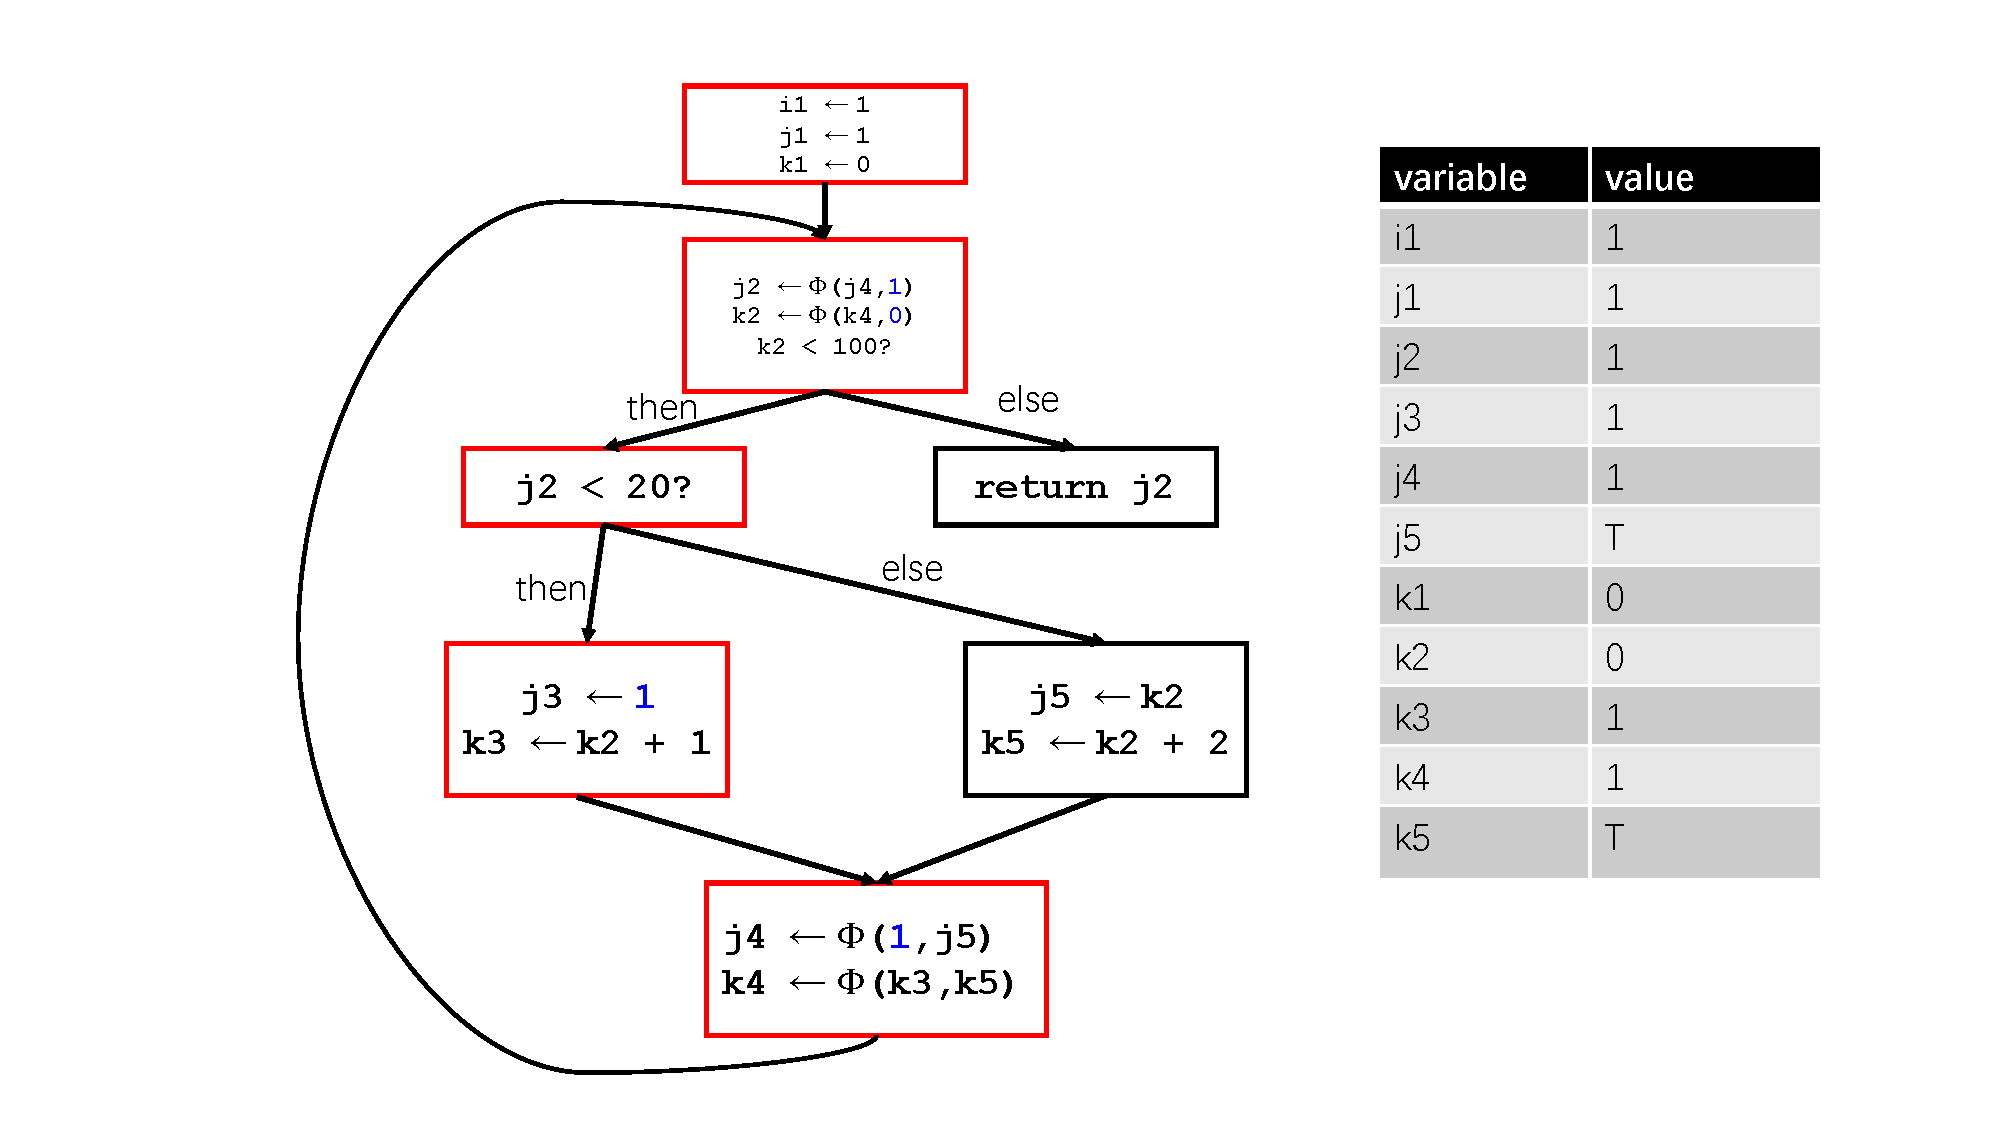
\includegraphics[width=\textwidth]{p49.pdf}
%          \caption{Code after moving instruction.}
%          \label{fig:p49}
%      \end{subfigure}
%           \begin{subfigure}{0.6\textwidth}
%      \centering
%          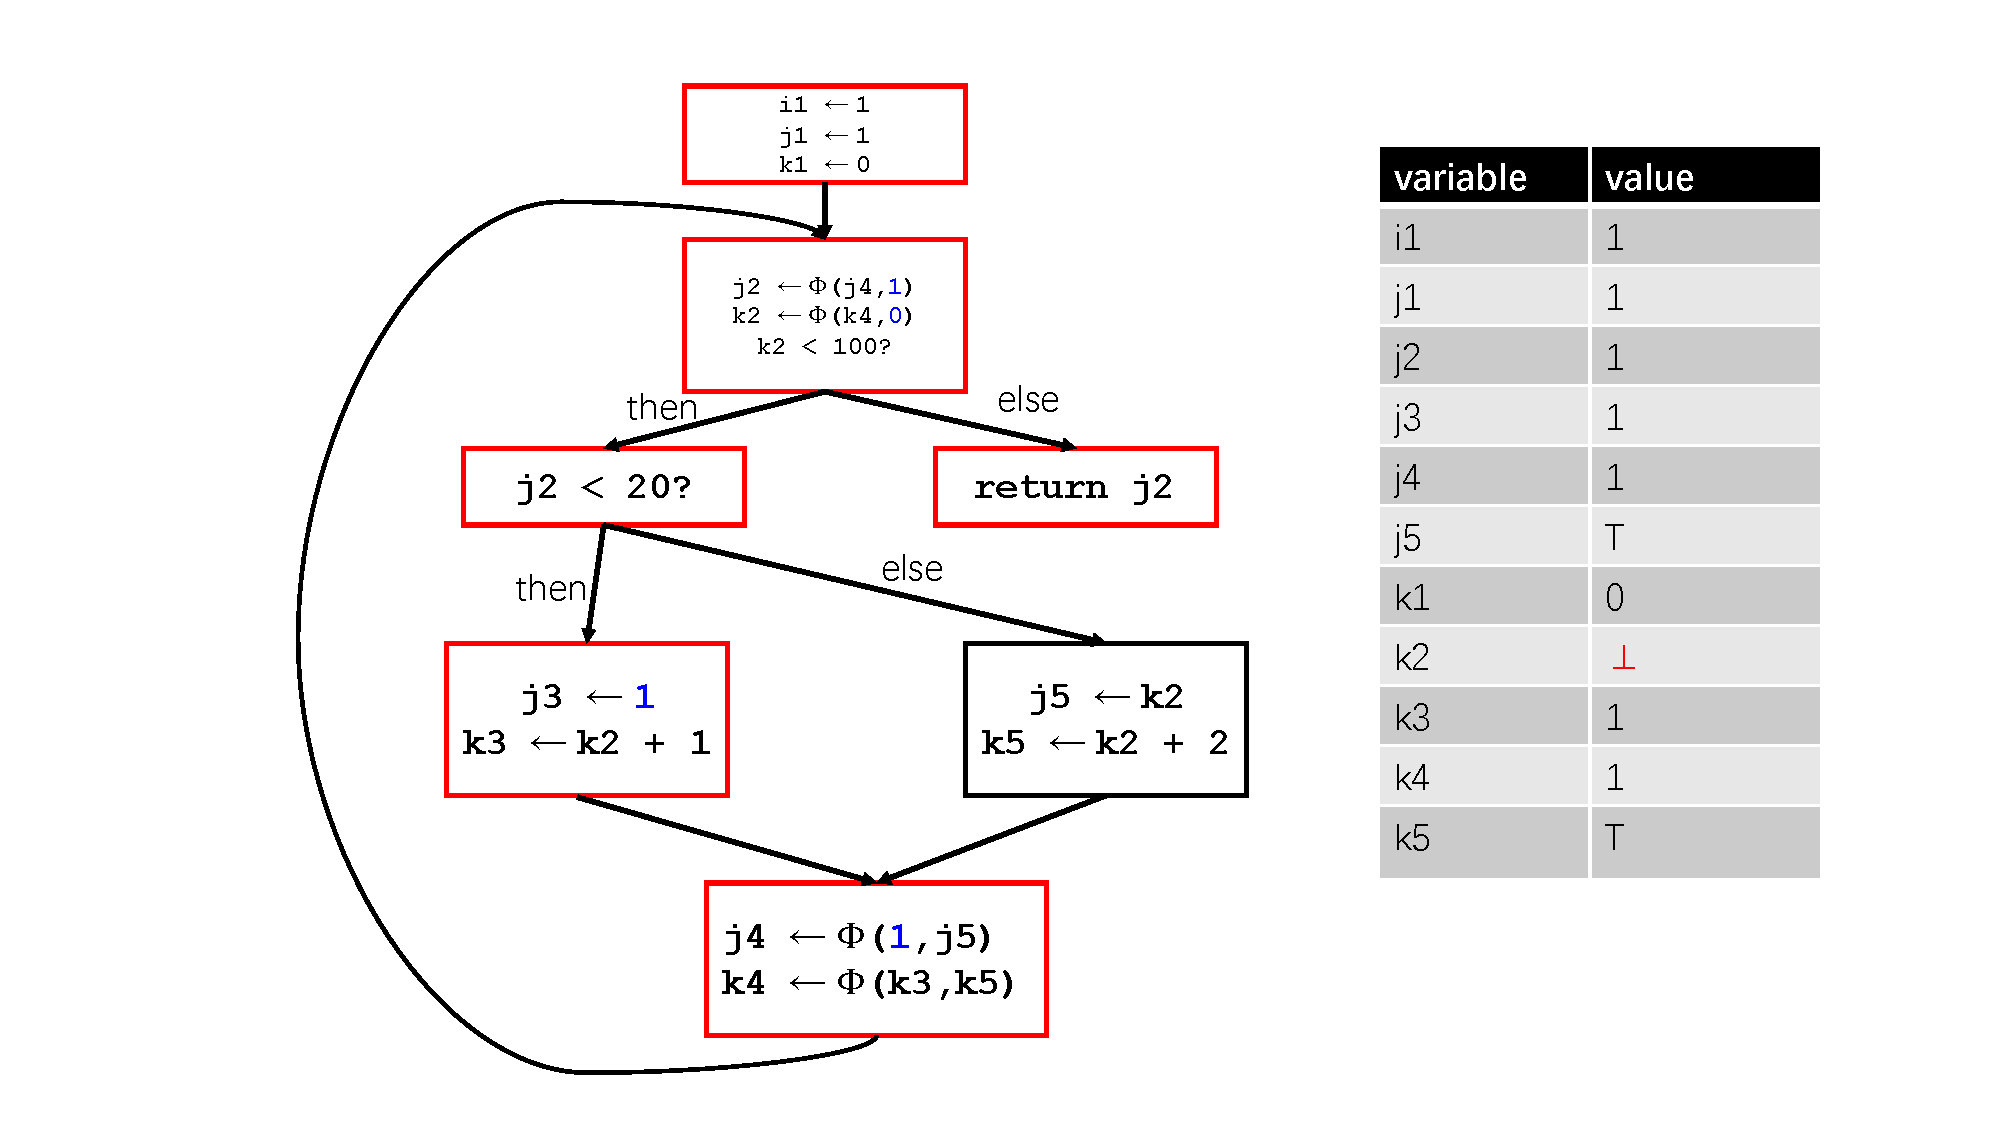
\includegraphics[width=\textwidth]{p50.pdf}
%          \caption{Code after moving instruction.}
%          \label{fig:p50}
%      \end{subfigure}
%           \begin{subfigure}{0.6\textwidth}
%      \centering
%          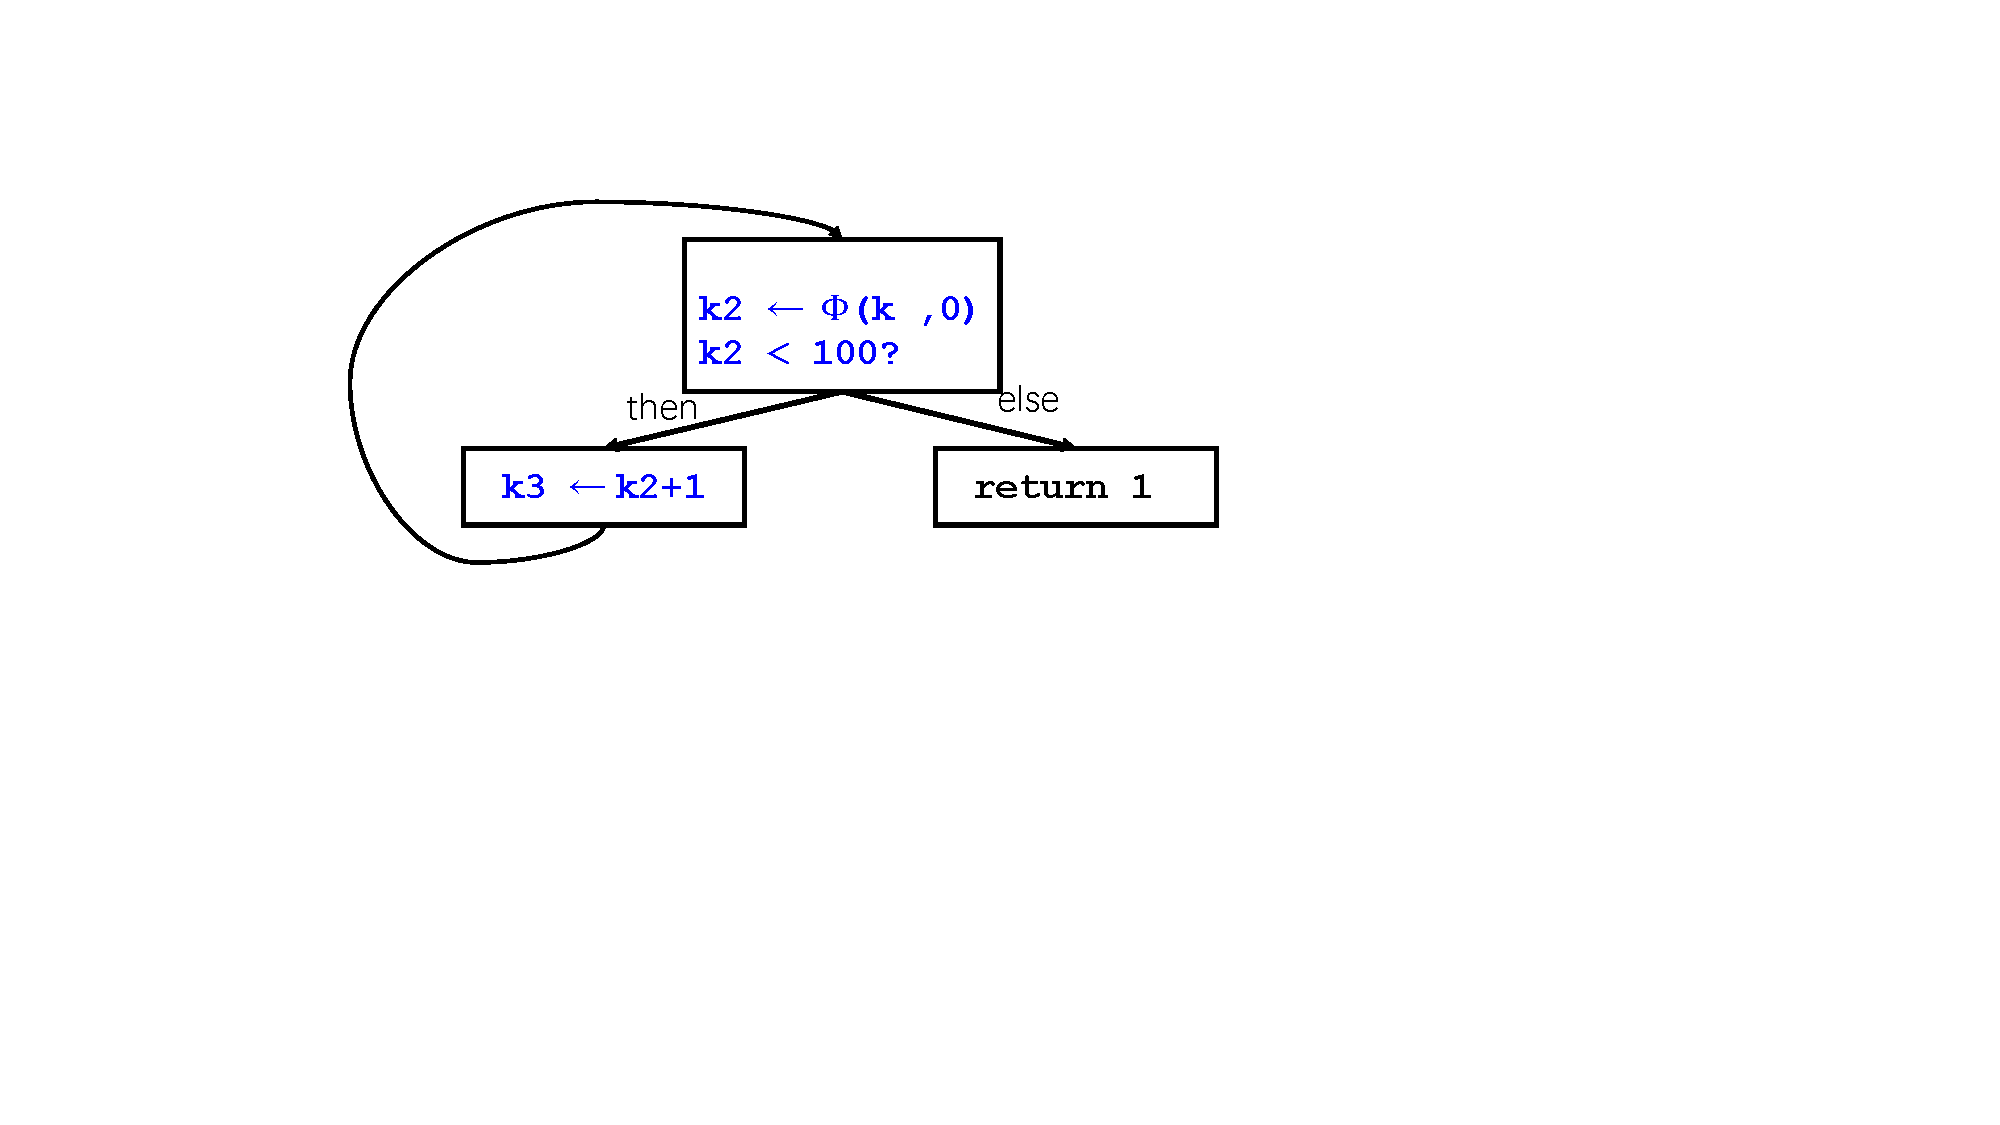
\includegraphics[width=\textwidth]{p51.pdf}
%          \caption{Code after moving instruction.}
%          \label{fig:p51}
%      \end{subfigure}
%         \caption{Implementing $\Phi$-function}
%         \label{fig:p47-51}
% \end{figure}




\subsection{Copy Propogation}

\begin{note}{notes}
	\begin{itemize}
		\item  delete x $\gets \Phi$ (y,y,y) and replace all x with y
		\item delete x $\gets$ y and replace all x with y
	\end{itemize}
\end{note}



\subsection{Aggressive Dead Code Elimination}

We can easily define the standard algorithm \ref{alg:Dead Code Elimination} below, but this algorithm may leave zombies.
Look at the example in Figure \ref{fig:p55-56}


\begin{algorithm}[H]
	\caption{Dead Code Elimination}\label{alg:Dead Code Elimination}
	\begin{algorithmic}
		\State {W $\gets$  list of all defs}
		\While{!W.isEmpty}
		\State{Stmt S $\gets$ W.removeOne}
		\If{$|S.users| != 0$}
		\State{\textbf{continue}}
		\EndIf
		\If{S.hasSideEffects()}
		\State{\textbf{continue}}
		\EndIf
		\For {def in S.operands.definers}
		\State{def.users $\gets$ def.users - \{S\}}
		\If{$|def.users| == 0$}
		\State{W $\gets$ W UNION \{def\}}
		\EndIf
		\EndFor
		\State{delete S}
		\EndWhile
	\end{algorithmic}
\end{algorithm}


\begin{figure}[H]
	\centering
	\begin{subfigure}{0.4\textwidth}
		\centering
		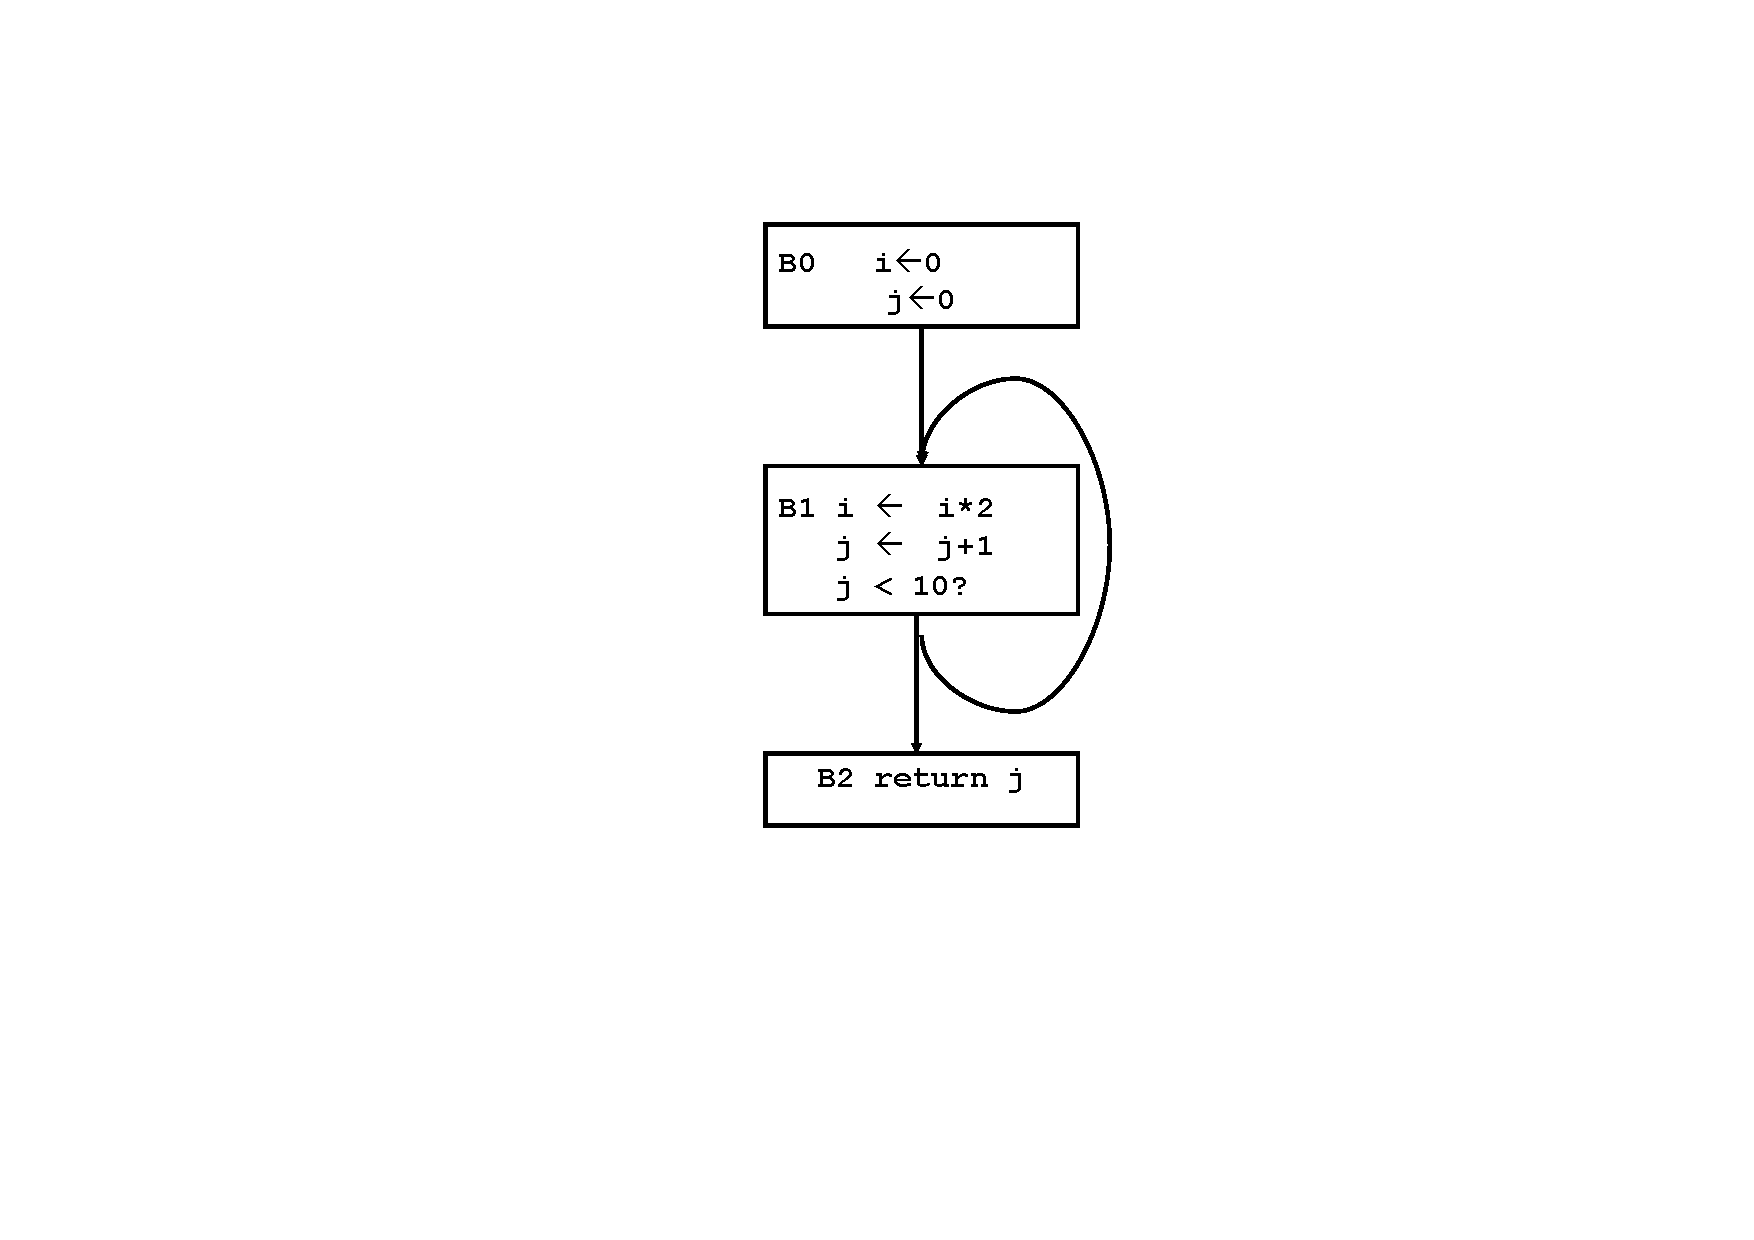
\includegraphics[width=\textwidth]{p55.pdf}
		\caption{Original code. We can easily find that instructions relating to $i$ are dead and can be eliminated.}
		\label{fig:pp55}
	\end{subfigure}
	\begin{subfigure}{0.4\textwidth}
		\centering
		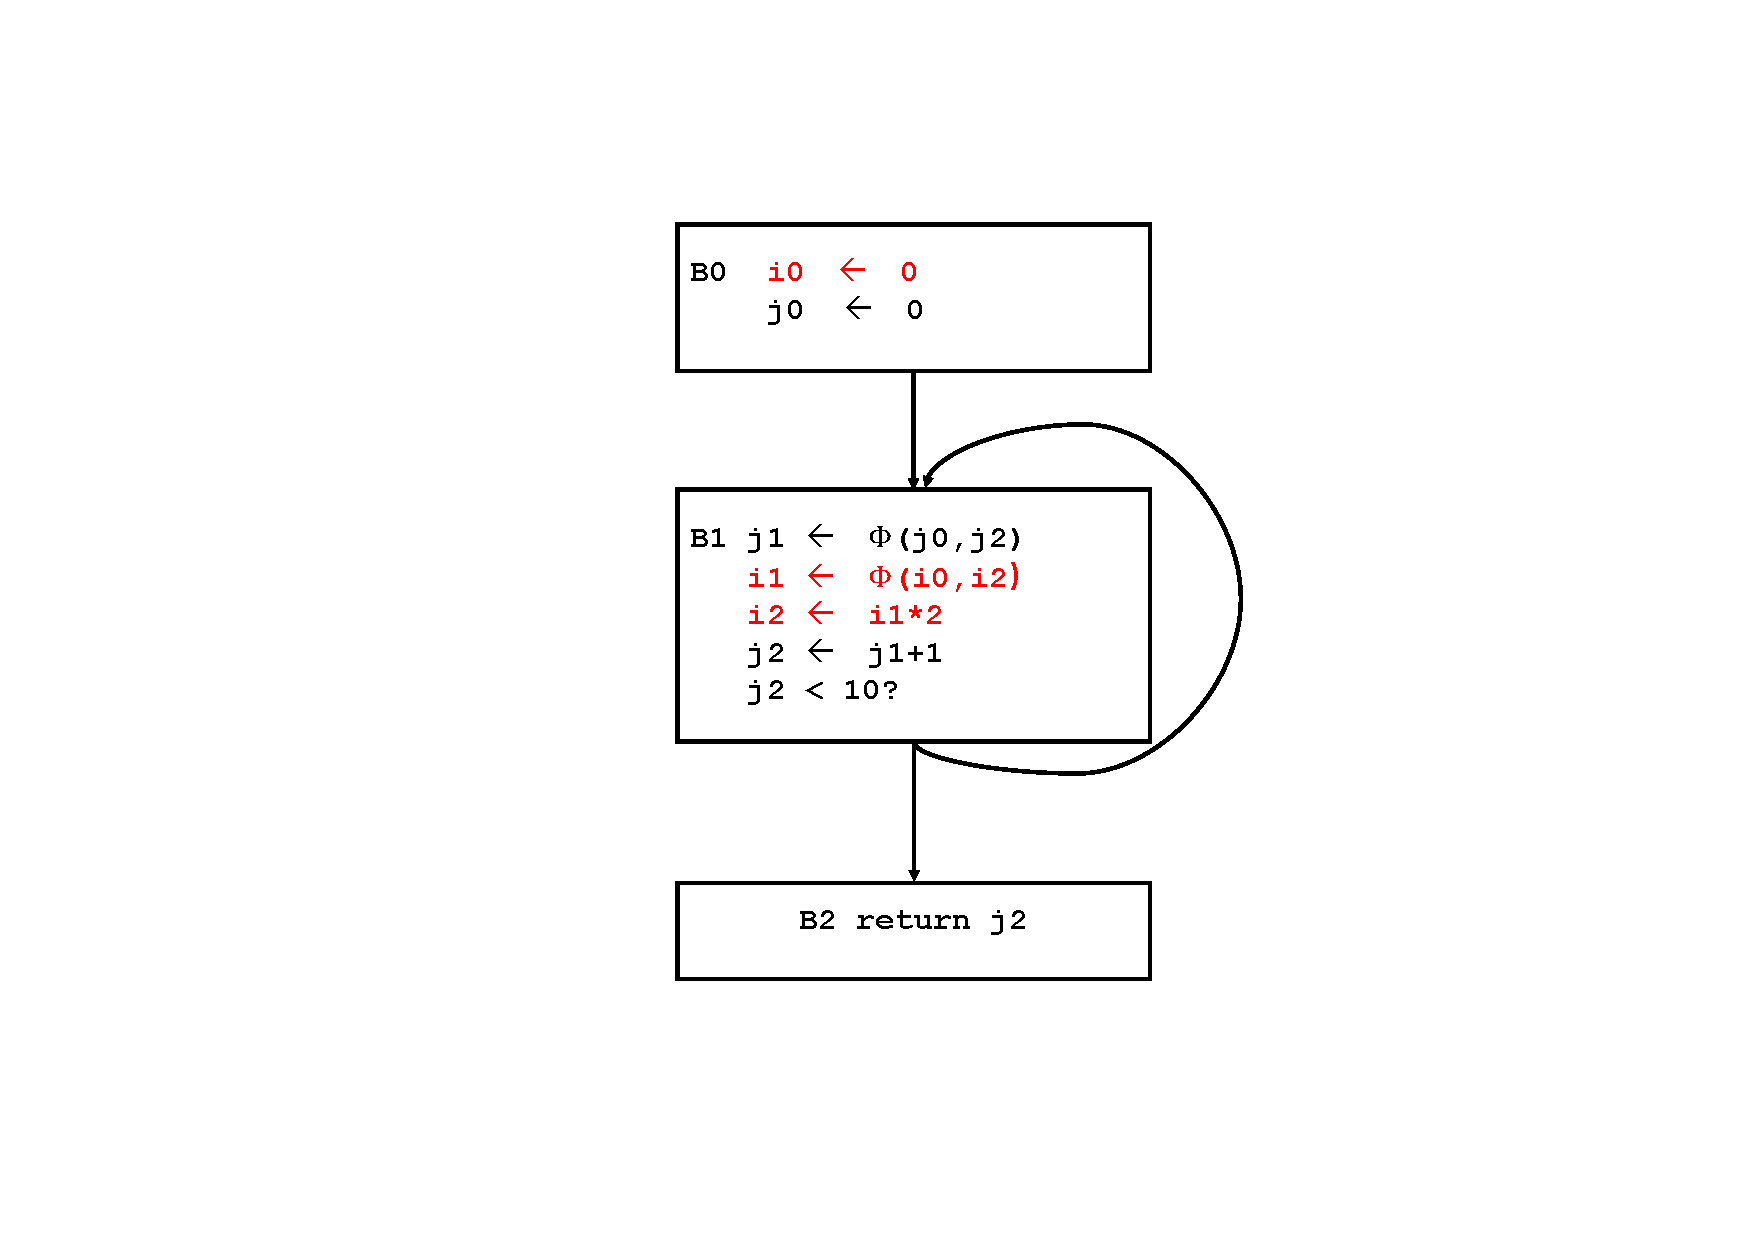
\includegraphics[width=\textwidth]{p56.pdf}
		\caption{SSA format code. Since there is a circle use chain so we can not remove instructions relating to $i$ because $i_1$ uses $i_2$, and $i_2$ uses $i_1$}.
		\label{fig:p56}
	\end{subfigure}


	\caption{An example to illustrate standard DCE can leave zombies.}
	\label{fig:p55-56}
\end{figure}

So instead of assuming everything is live until proven dead, we go another way: assuming everything is dead until proven live
shown in algorithm \ref{alg:Aggressive Dead Code Elimination}.



\begin{algorithm}[H]
	\caption{Aggressive Dead Code Elimination}\label{alg:Aggressive Dead Code Elimination}
	\begin{algorithmic}
		\Function{init}{}
		\State{mark as {\color{blue}live} all stmts that have side-effects:}
		\State{ \,\,\,\,\,\,\,\,    I/O}
		\State{  \,\,\,\,\,\,\,\,   stores into memory}
		\State{  \,\,\,\,\,\,\,\,   returns}
		\State{  \,\,\,\,\,\,\,\,   calls a function that MIGHT have side-effects}
		\State{As we mark S live, insert S.operands.definers into W}
		\While {$|W| > 0$}
		\State{S $\gets$ W.removeOne()}
		\If{{\color{blue}(S is live)}}
		\State{\textbf{continue}}
		\EndIf
		\State{{\color{blue}mark S live, insert S.operands.definers into W}}

		\EndWhile
		\EndFunction
	\end{algorithmic}
\end{algorithm}


\subsubsection{Problems within algorithm \ref{alg:Aggressive Dead Code Elimination}}
After Aggressive Dead Code Elimination applied to function  shown in \ref{fig:p58}, there is only one \texttt{return} statement left.
However, control flow is undecidable in general, so possibly the loop in \ref{fig:pp51} will iterate indefinitely and the \texttt{return } instruction will never be executed.
The problem here is we simply mark the branch statement dead.
\begin{figure}[H]
	\centering
	\begin{subfigure}{0.5\textwidth}
		\centering
		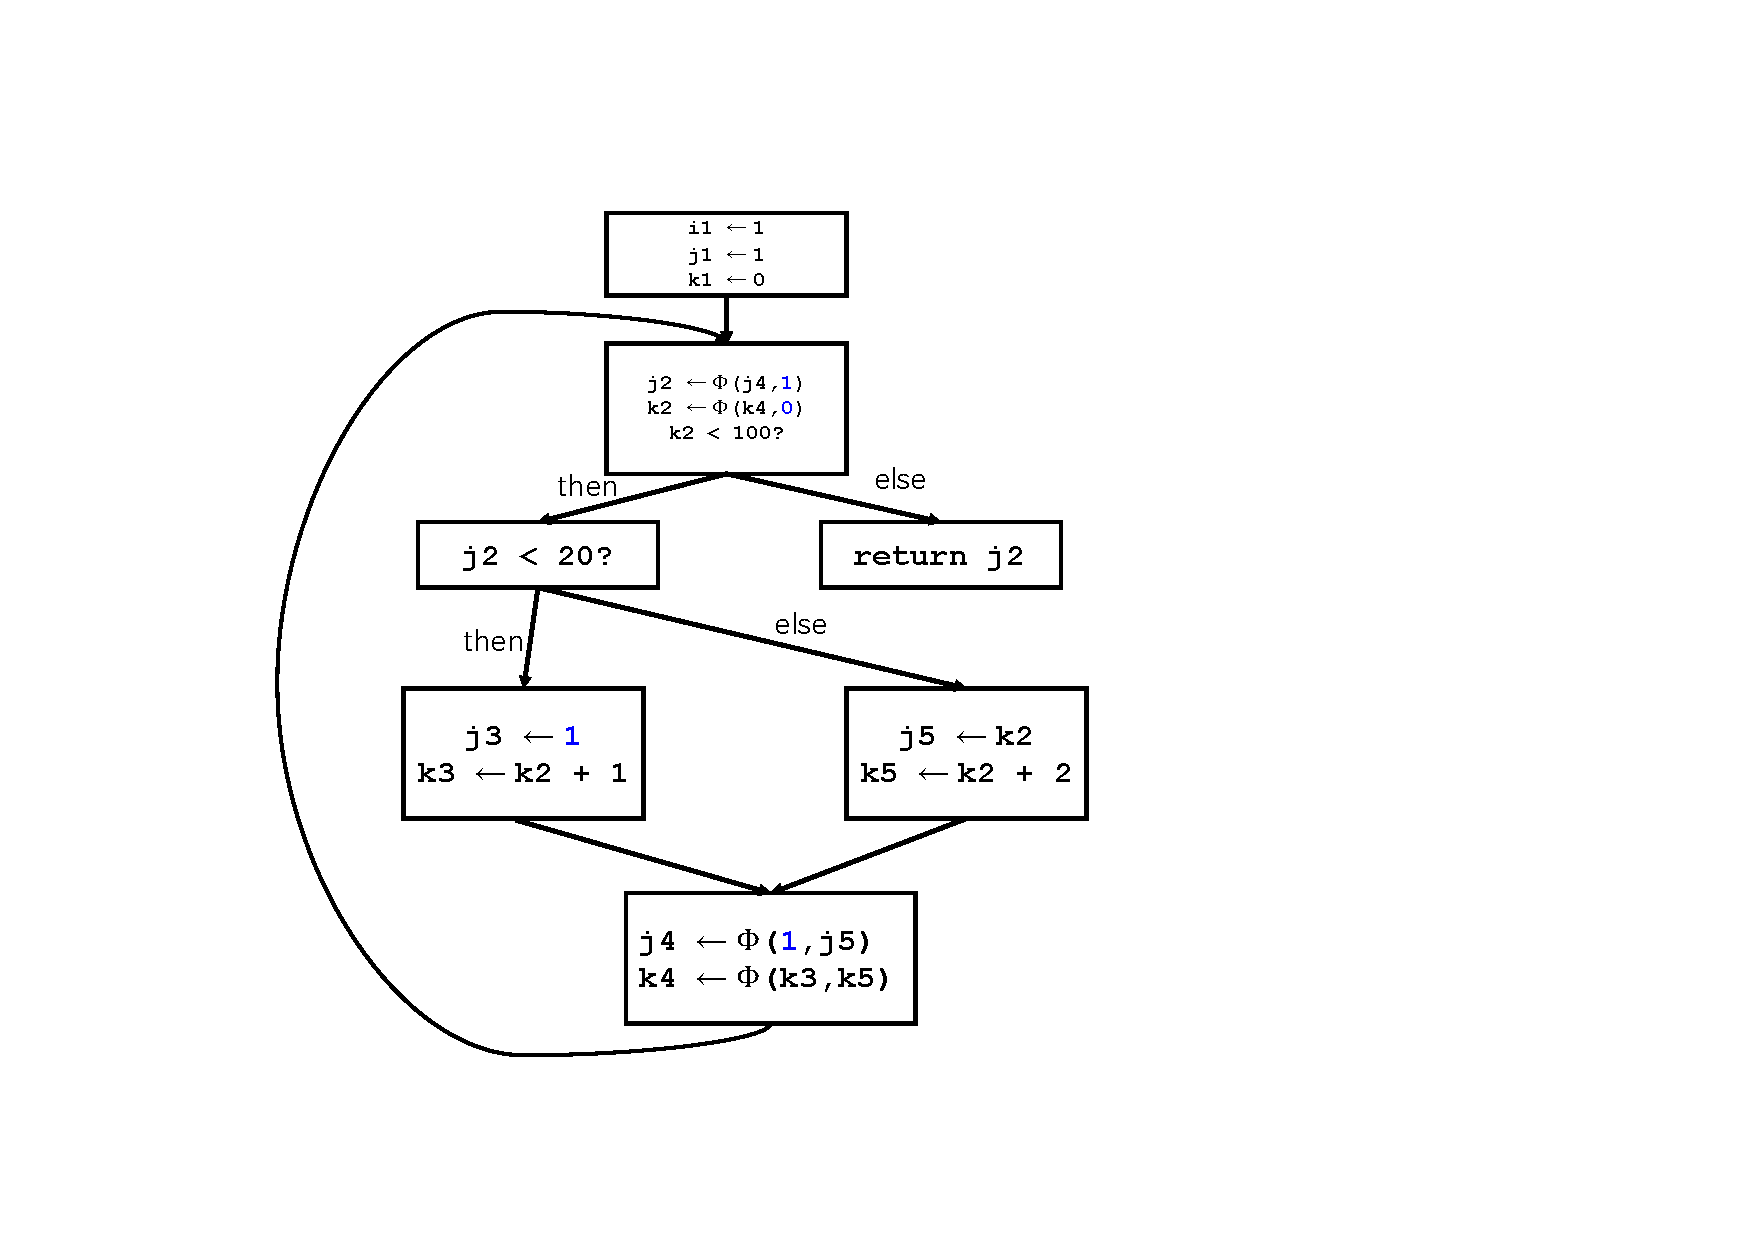
\includegraphics[width=\textwidth]{p58.pdf}
		\caption{Original code in SSA format. }
		\label{fig:p58}
	\end{subfigure}
	\begin{subfigure}{0.5\textwidth}
		\centering
		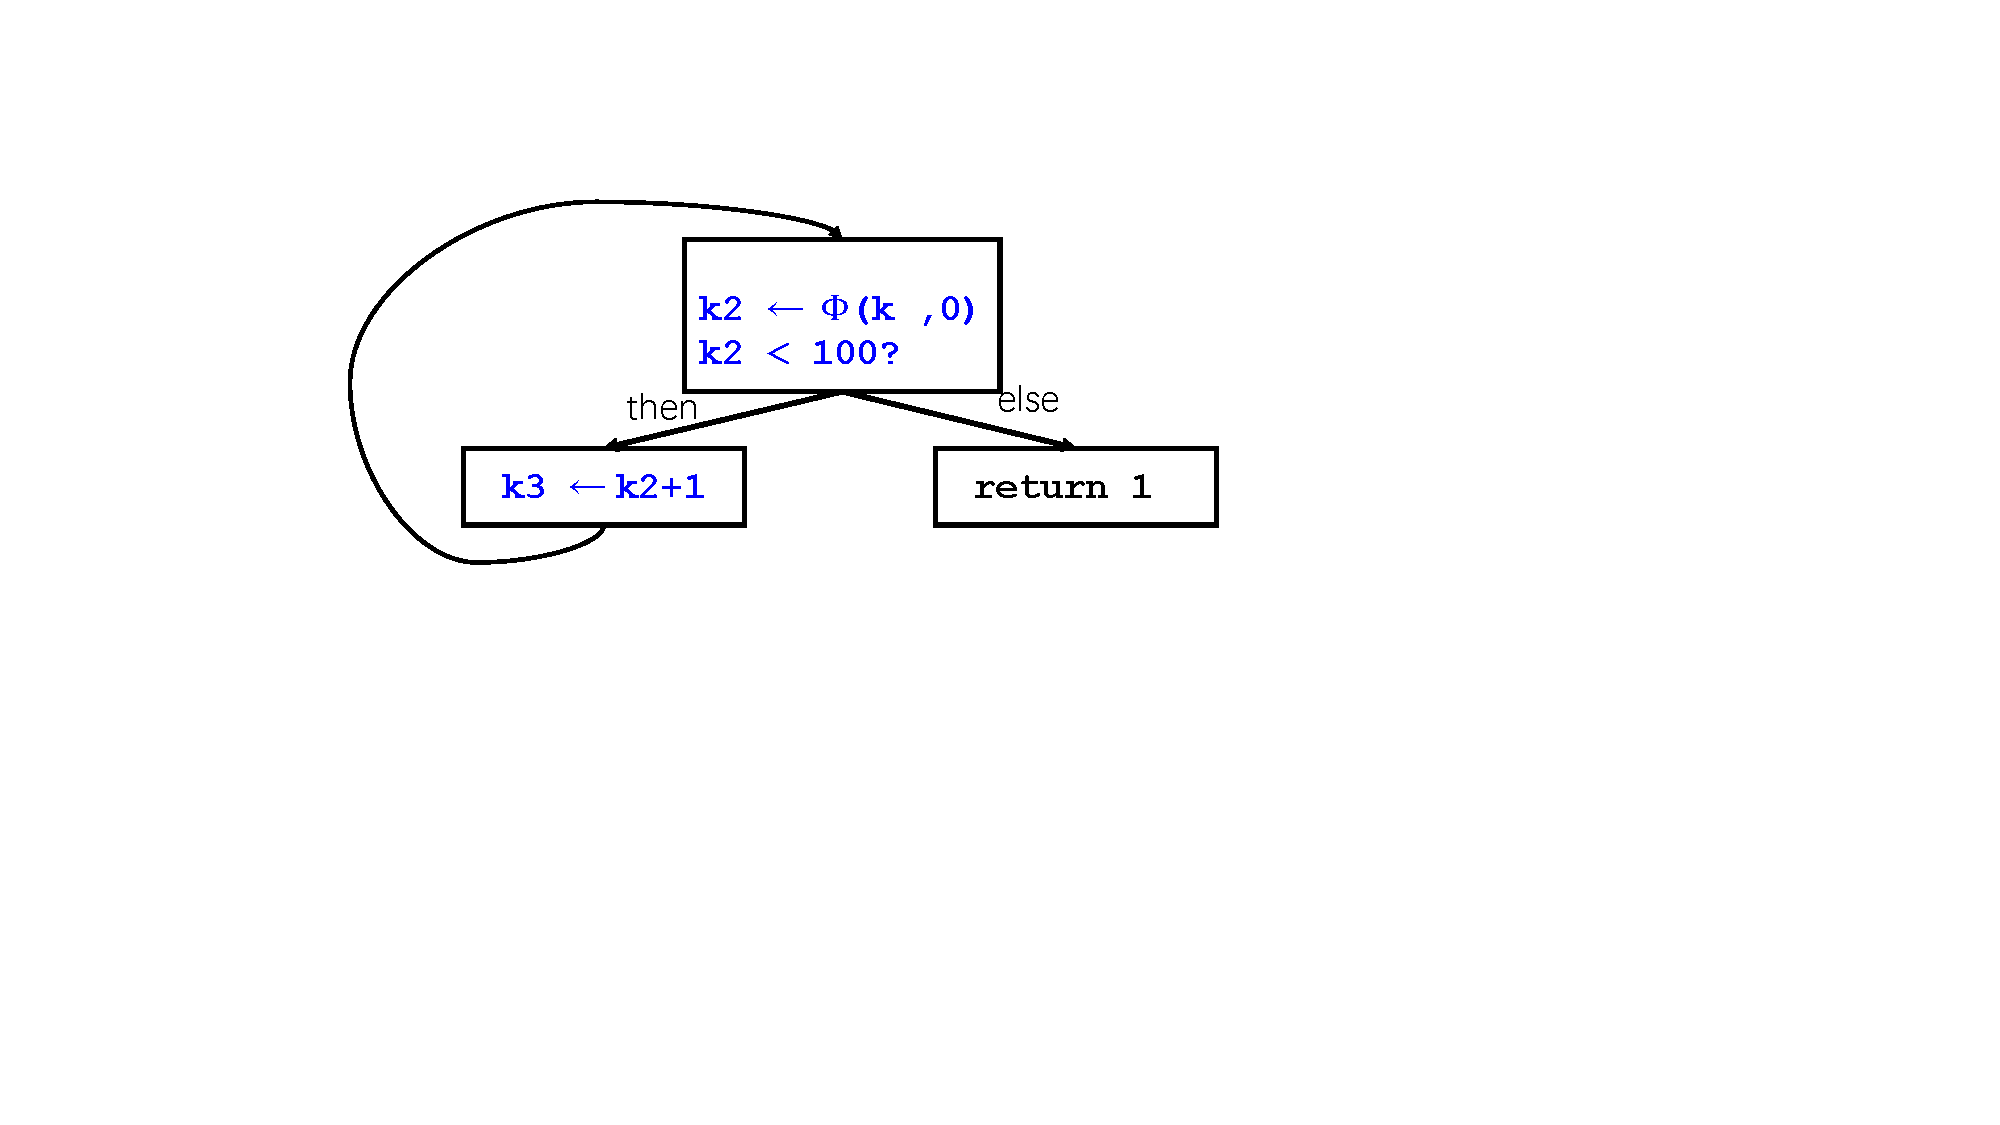
\includegraphics[width=\textwidth]{p51.pdf}
		\caption{After CCP}
		\label{fig:pp51}
	\end{subfigure}
	\begin{subfigure}{0.5\textwidth}
		\centering
		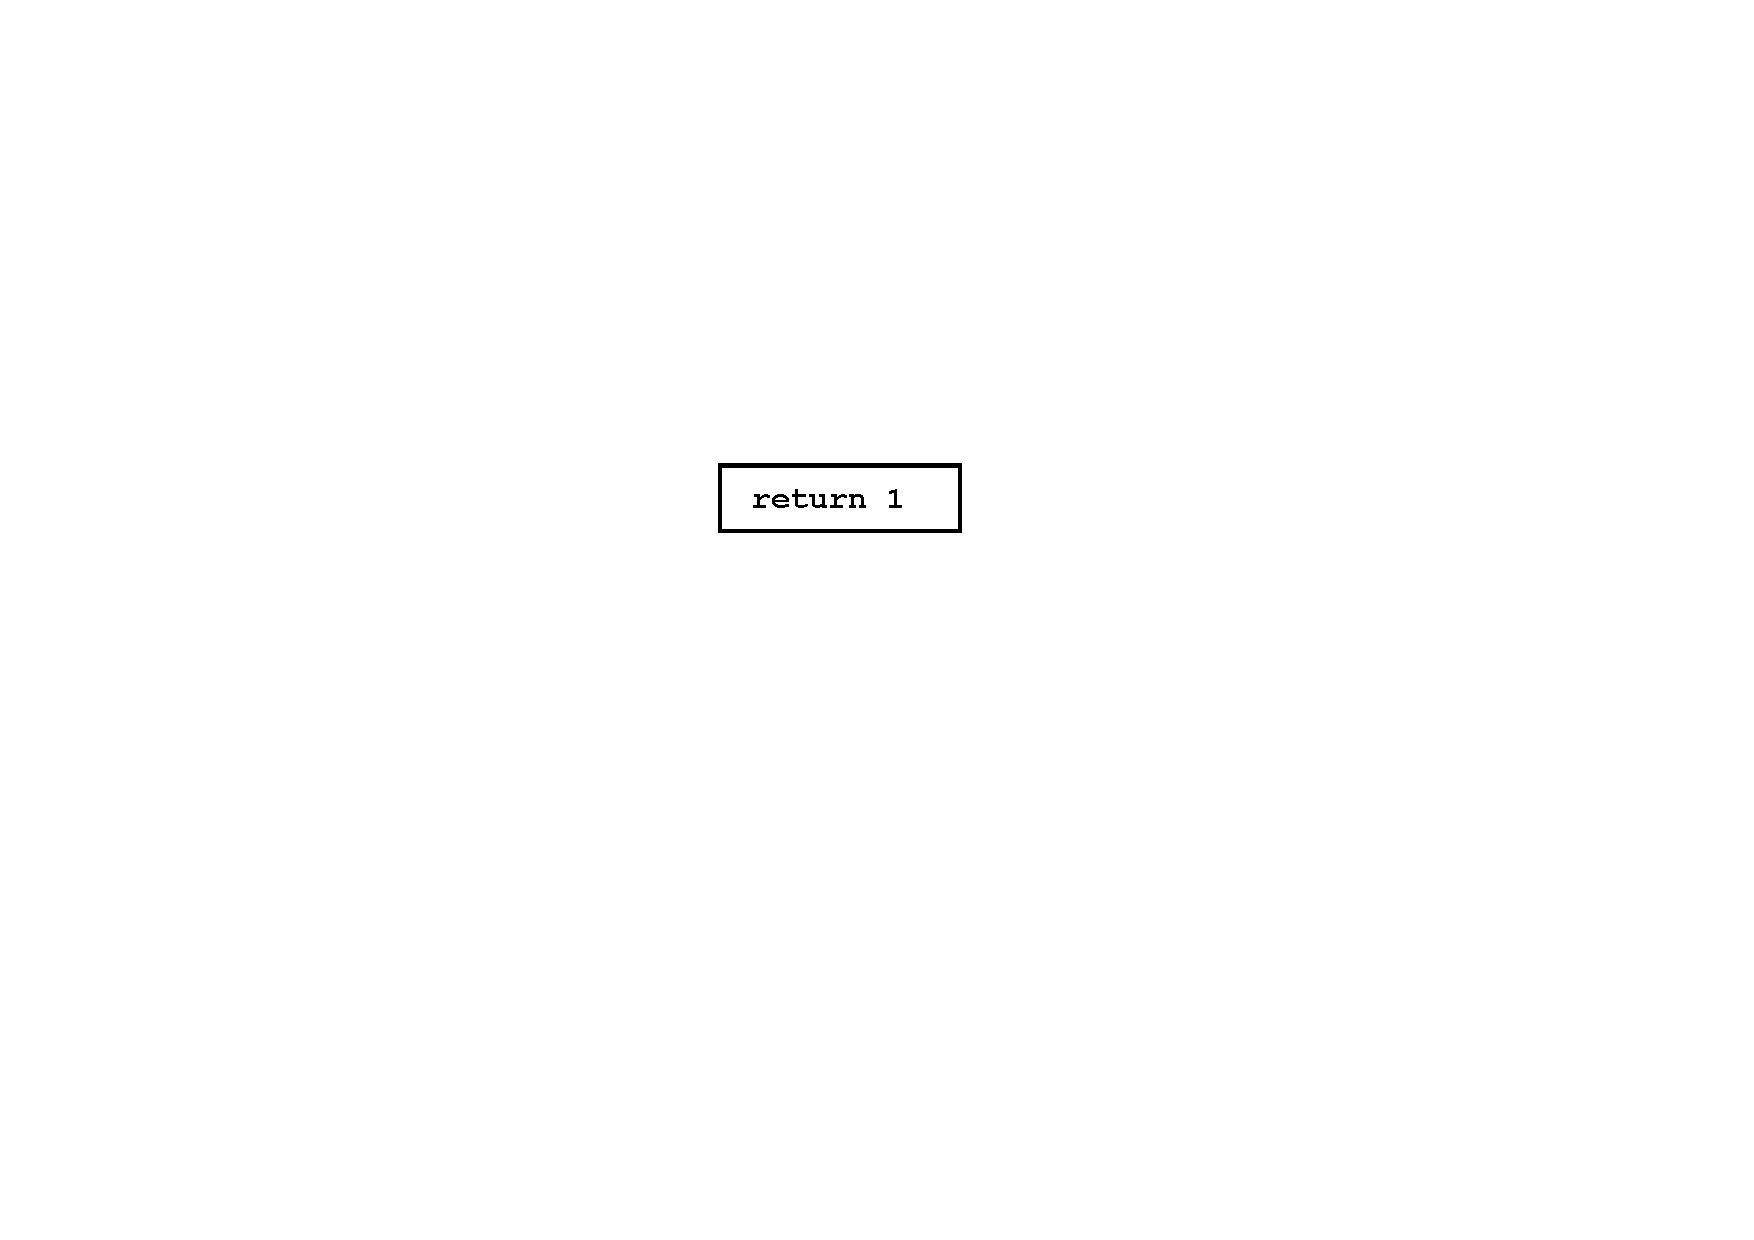
\includegraphics[width=\textwidth]{p57.pdf}
		\caption{After ADCE}
		\label{fig:p57}
	\end{subfigure}
	\caption{An example to illustrate the algorithm \ref{alg:Aggressive Dead Code Elimination} has a problem.}
	\label{fig:p51-58}
\end{figure}


Also when we apply this algorithm to \ref{fig:p55-56}, we can find that \texttt{j2 < 10} is marked dead which is wrong. Of course,
we can simply mark all branches live in the initialize stage, but this is not the ideal solution.


Now we need to carefully consider which conditional branches need to be marked live.



\subsubsection{Control Dependence}

\begin{definition}{control dependence}
	Y is control-dependent on X if
	\begin{itemize}
		\item X branches to u and v
		\item $\exists$ a path u $\rightarrow$ exit which does not go through Y
		\item $\forall$ paths v  $\rightarrow$ exit go through Y
	\end{itemize}
	This means X casn determine whether or not Y is executed.
	\begin{figure}[H]
		\centering
		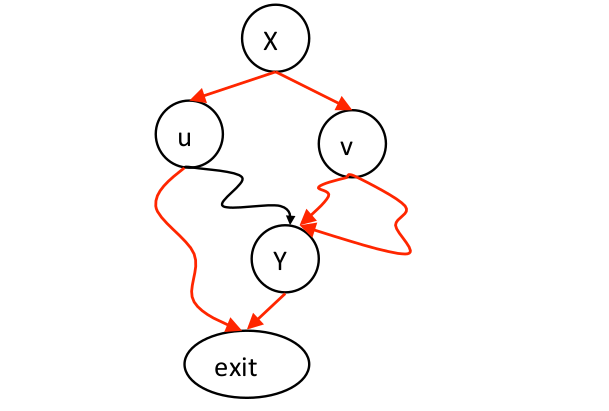
\includegraphics[width=0.5\textwidth]{p59.png}

	\end{figure}
\end{definition}


\subsubsection{Aggressive Dead Code Elimination(Fixed Version)}

So we make a little modification \ref{alg:Aggressive Dead Code Elimination(Fixed Version)}. When we mark S is live, we should also mark live those conditional branches upon which S is
control dependent.

\begin{algorithm}[H]
	\caption{Aggressive Dead Code Elimination(Fixed Version)}\label{alg:Aggressive Dead Code Elimination(Fixed Version)}
	\begin{algorithmic}
		\Function{init}{}
		\State{mark as live all stmts that have side-effects:}
		\State{ \,\,\,\,\,\,\,\,    I/O}
		\State{  \,\,\,\,\,\,\,\,   stores into memory}
		\State{  \,\,\,\,\,\,\,\,   returns}
		\State{  \,\,\,\,\,\,\,\,   calls a function that MIGHT have side-effects}
		\State{As we mark S live, insert S.operands.definers into W}
		\State{\color{red} S.CD$^{-1}$ into W}
		\While {$|W| > 0$}
		\State{S $\gets$ W.removeOne()}
		\If{(S is live)}
		\State{\textbf{continue}}
		\EndIf
		\State{mark S live, insert S.operands.definers into W}
		\State{\color{red} S.CD$^{-1}$ into W}
		\EndWhile
		\EndFunction
	\end{algorithmic}
\end{algorithm}



\subsubsection{Finding the Control Dependence Graph}

\begin{itemize}
	\item Construct CFG
	\item Add entry node and exit node
	\item Add (entry, exit) edge
	\item Create G$^\prime$, the reverse CFG
	\item Compute D-tree in G$^\prime$ (post-dominators of G)
	\item Compute DF$_G^\prime$(y) for all y $\in$ G$^\prime$ (post-DF of G)
	\item Add (x,y)$\in$ G to CDG if x $\in$ DF$_G^\prime$(y)
\end{itemize}



So let us calculate the control dependence for Figure \ref{fig:pp55} which is shwon in Figure \ref{fig:p60}. Since Block1 is control dependent on Block1, so the conditional
branch in Block1 \texttt{j2 < 10 ?} should be marked live now.

\begin{figure}[H]
	\centering
	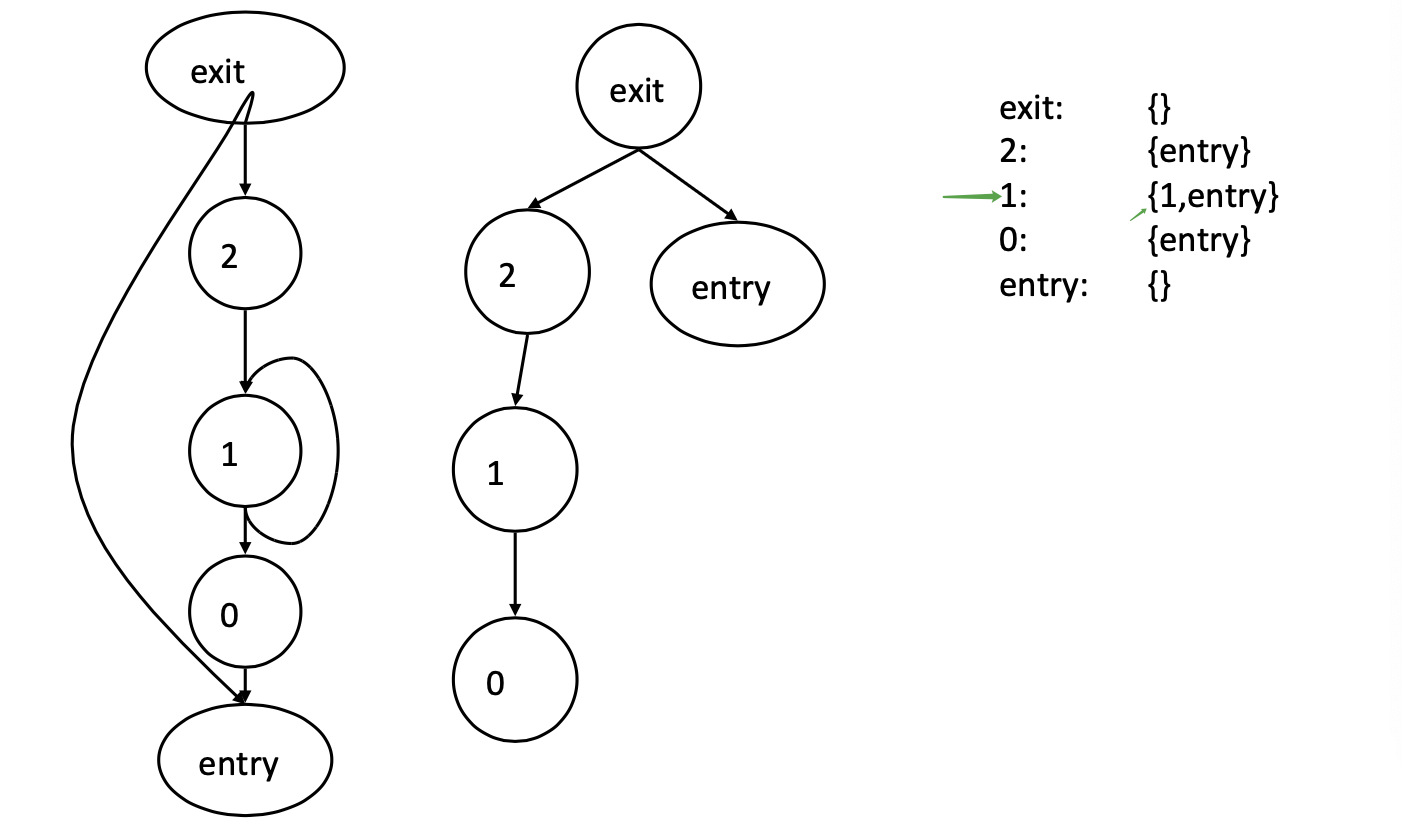
\includegraphics[width=0.6\textwidth]{p60.png}
	\caption{From left to right are G$\prime$, post-dominators of G and post-DF of G respectively.}
	\label{fig:p60}
\end{figure}



